\documentclass[10pt,a4paper,twocolumn]{article}
\usepackage{bachelorproject}
\usepackage{hyperref}

% for the tables: https://www.latex-tables.com/
\usepackage{multirow}
\usepackage{colortbl}
\usepackage{booktabs}

\title{\vspace{-0.5in}{\bfseries\scshape
    % Using ensembles to address Bootstrapping Errors in Offline
    % Reinforcement Learning
    Addressing Bootstrapping Errors in Offline Reinforcement Learning
    with Ensembles
    } \\
    \vspace{1ex}
    \normalsize{Bachelor's Project Thesis}\vspace{-2ex}
}

\author{
    \normalsize{Marco Andrea Gallo, s3680622, m.a.gallo@student.rug.nl} \\
    \normalsize{Supervisor: Dr. Matthia Sabatelli}
}

\date{\vspace{-5ex}}


\begin{document}

\twocolumn[
  \maketitle
  \begin{@twocolumnfalse}
    \begin{abstract}
{TODO\vspace{6ex}}
\end{abstract}

  \end{@twocolumnfalse}
]

\thispagestyle{firststyle}

% FIXME there is a break-line somewhere after the second paragraph that
% appears idk why
% TODO read all again once the other subsections are defined, and
% evaluate what is written here. Should it be split up? Is the story
% coherent, are there no logical gaps and - especially, this is a
% mistake you tend to make - are you giving too much for granted without
% explaining it?
% TODO proof-read and understand: should I really have 2 RQs, or is it
% better to keep one and have the section on offline BE on DQV(Max) as
% some sort of preliminary results?
\section{Introduction}\label{sec:introduction}
% TS: advancements in ML are data-driven, we need the same for RL - can
% achieve it with offline RL
% NOTE could add some more references?
% NOTE shorten or split into sub-paragraphs, ca. 100w each
In the past decade, machine learning methods have encountered
major success over a wide number of real-world applications, ranging
from Computer Vision to Natural Language Processing tasks.
Much of the progress in these areas can be attributed to the
development of \textit{data-driven}, scalable learning methods. In
fact, although advancements in models and architectures are an integral
part of this success story, the learning techniques they employ are
well-founded and understood, and major improvements in model
performance stem from the availability of large and diverse training
datasets.
However, such data-driven methods do not map to the Reinforcement
Learning (RL) framework equally well. RL involves sequential decision
making problems where the best behavior strategy is learned through
active interaction with the environment. This naturally
\textit{online} learning paradigm prevents effective exploitation of
the rich \textit{offline} datasets, which is at the base of the
success of supervised learning methods.
Moreover, data collection for complex real-world RL applications such as
autonomous driving or healthcare support systems can often be
expensive or hazardous. Developing safe and capable
offline RL agents has therefore a great appeal: by efficiently
learning from large amounts of data, we could create ``generalizable
and powerful \textit{decision making engines}''
\citep{levine2020offline} that can aid in solving many real-world open
problems \citep{levine2020offline}.

% TS: offline RL entails reasoning about what has not happened
% (counterfactual queries); this is problematic for standard ML and
% creates distribution shift DS
In offline RL, an agent learns a policy from a static dataset of
logged experiences produced by a \textit{behavior policy}.
This differs from classical online RL, where an agent can actively
collect new experience by interacting with its environment
\citep{sutton2018reinforcement}. For an offline agent to
improve, it is therefore crucial that it is able to partake in
counterfactual
reasoning to accurately estimate what would happen if it took a
decision different from the one in the training dataset
\citep{levine2020offline}. By contrast, an online RL agent could
explore and learn on its own the effects of a decision
different than the one previously chosen in the same situation. This
additional constraint of offline RL is
problematic, and it exceeds the capabilities of current machine learning
methods that use expressive function approximators (neural networks)
to generalize across examples. For one, it violates the assumption of
independent and
identically distributed data (i.i.d.) that standard supervised
learning algorithms rely on: an offline RL agent may be trained under
one distribution but tested under a different one.
In addition, an offline agent must be able to reason differently from
the data-generating policy in order to produce novel -- and possibly
favorable -- courses of actions; this requirement breaks the i.i.d.\
assumption too.
The mismatch between the behavior policy-induced distribution and the
one learned during training is called \textit{distributional shift},
and it presents a fundamental challenge for the efficacy of offline RL
\citep{levine2020offline}.

% TS: DS affects online and offline off-policy algos, especially in
% the form of bootstrapping error
Distributional shift generally affects off-policy RL algorithms. These
are methods that learn about a \textit{target policy} using a
different \textit{behavior policy} \citep{sutton2018reinforcement},
such as the popular Q-learning agent \citep{watkins1992q}. Due to
their ability to learn from data generated by another policy,
off-policy algorithms naturally lend themselves to offline RL.\@ It is
well known that off-policy methods exhibit high variance
\citep{sutton2018reinforcement}; moreover,
off-policy algorithms which employ a maximization operation in the
bootstrapping step, such as Q-learning,
are prone to overoptimistic value estimates
\citep{thrun1993issues}. In the offline setting, this form of
\textit{bootstrapping error} results in the selection of actions that
lie outside of the training data distribution
\citep{kumar2019stabilizing}, and since no ground truth information to
estimate their value is available - the dataset is fixed - they
disrupt the training process and drive it towards regions of
uncertainty; a more in-depth account of the bootstrapping error
follows in Section~\ref{sec:BE}.

% NOTE look at commented part at end of paragraph for another
% formulation of RQ
% TS: ensemble methods address the bootstrapping error, off-policy and
% offline generally; do the results related to standard Deep
% Q-Learning with ensembles transfer to other value-based methods,
% such as DQV family?
To address distributional shift and bootstrapping errors in
off-policy learning, many techniques found in the literature employ
ensemble-based methods (\citeauthor{osband2016deep},
\citeyear{osband2016deep}; \citeauthor{anschel2017averaged},
\citeyear{anschel2017averaged}; \citeauthor{pmlr-v97-fujimoto19a},
\citeyear{pmlr-v97-fujimoto19a}, appendix D.2).
% \citep{osband2016deep, anschel2017averaged,
%   pmlr-v97-fujimoto19a}.
Most relevant for this research,
ensembling methods have demonstrated a successful approach in
offline RL, as seen in the REM agent by
\citet{agarwal2020optimistic}. This
paper investigates to which extent results concerning bootstrapping
error prevention based on ensembled versions of Q-learning transfer to
other model-free, value-based RL algorithms in the context of offline
RL.\@ In particular, we will inquire whether benefits concerning
bootstrapping error reduction stemming from simple ensembling methods
apply to the deep RL agents of the DQV algorithmic family
\citep{sabatelli2020deep}.
% also apply to RL algorithms that already take steps to minimize it,
% such as the DQV algorithmic family \citep{sabatelli2020deep}.

\subsection{Background}
The following subsections will introduce some definitions and prior
knowledge needed to understand this paper.

% NOTE expressed the set of actions w/out a time subscript on the
% actions assuming that all actions are available at all states
% NOTE using R(s,a) as reward signal instead of R_t in order to avoid
% explaining it is a random variable, the explanation seems more
% straightforward in this way to me
% TODO should I write more of the presented equations in a an \equation
% environment? Check that later, keep it tightly spaced for now
\subsubsection{Reinforcement Learning}\label{sec:RL_BG}
% TS: RL general elements
Reinforcement Learning seeks to solve a Markov Decision Process
(MDP) ($\mathcal{S},\mathcal{A},p,R$). In
RL, an agent interacts with an environment at
discrete time steps $t=0,1,2,3,\ldots$. At each time step $t$, the
agent receives a representation of the environment $s_t \in
\mathcal{S}$, on which it can perform some action $a_t \in
\mathcal{A}(s)$ that determines its transition to a new state
$s_{t+1}$ according to the dynamics model
$p\colon\mathcal{S}\times\mathcal{S}\times\mathcal{A}\rightarrow
\left[0,1\right],p\left(s^\prime\mid
  s,a\right)\doteq\Pr\left\{s^\prime=s_{t+1}\mid
  s=s_t,a=a_t\right\}$. Following this transition, the agent receives
reward $r_{t+1}$ from a reward function
$R\colon\mathcal{S}\times\mathcal{A}\rightarrow\mathbb{R},
r_{t+1}=R\left(s_t,a_t\right)$. The goal of a RL agent is then to find
a mapping from states to action probabilities, called a \textit{policy}
$\pi\colon\mathcal{S}\times\mathcal{A}\rightarrow\left[0,1\right],
\pi\left(a\mid s\right)=\Pr\left\{a_t=a,s_t=s\right\}$, which
maximizes the \textit{expected return} $G_t\doteq
\sum_{t=0}^{\infty}\gamma^{t}R\left(s_t,a_t\right)$ where
$\gamma\in\left[0,1\right]$ is a discount factor used to scale the
importance of future rewards. Each policy $\pi$ has a matching
\textit{state value function}
$V^{\pi}\left(s\right)=\mathbb{E}\left[G_t\mid s=s_t\right]$, which
indicates the expected return obtained starting from state $s$ therefore
following $\pi$. This function can also be expressed in terms of
state-action pairs as a \textit{state-action value function}
$Q^{\pi}\left(s,a\right)=\mathbb{E}\left[G_t|s=s_t,a=a_t\right]$,
indicating the expected return taking action $a$ in state $s$ and
consequently following $\pi$. Altogether, the RL optimization problem aims
to achieve a policy $\pi^*$ characterized by the \textit{optimal Q
  value function}
$Q^*\left(s,a\right)\doteq\max_{\pi}Q^{\pi}\left(s,a\right)$ for all
$s\in\mathcal{S}$ and $a\in\mathcal{A}\left(s\right)$, whose solution
is provided by the Bellman optimality equation
\begin{equation}
\begin{aligned}
Q^*\left(s_t,a_t\right)=\mathbb{E}\bigg[&R\left(s_t,a_t\right)+\\ &\gamma
  \max_{a\in\mathcal{A}\left(s\right)}Q^*\left(s_{t+1},a\right)\bigg\vert
  s_t=s,a_t=a \bigg]
\end{aligned}
\end{equation}
\citep{bellman1957dynamic}. Note that the latter can
also be expressed as the \textit{optimal state value function}
$V^*\left(s\right)$ replacing the optimal $Q$ value estimate at
the next state
$\max_{a\in\mathcal{A}\left(s\right)}Q^*\left(s_{t+1},a\right)$ by
$V^*\left(s_{t+1}\right)$.

% TS: Deep RL and Q-learning
$Q^*\left(s,a\right)$ and $V^*\left(s\right)$ can both be learned by
Temporal Difference (TD) learning
\citep{sutton1988learning}. Q-learning is probably the most popular TD
method; it learns the state-action value function using the update
rule
\begin{equation}
Q\left(s_t,a_t\right)\leftarrow
Q\left(s_t,a_t\right)+\alpha\left[R\left(s_t,a_t\right)+y^{\scriptscriptstyle
TD}_{\scriptscriptstyle QL}\right],
\end{equation}
where
\[
y^{\scriptscriptstyle TD}_{\scriptscriptstyle
QL}=\gamma\max_{a\in\mathcal{A}\left(s\right)}Q\left(s_{t+1},a\right)-Q\left(s_t,a_t\right)
\]
\citep{watkins1992q}. When the state space $\mathcal{S}$ is large and
high dimensional, the $Q$ function is approximated by expressive
neural networks and we talk of Deep Reinforcement Learning
(DRL). DRL agents such as Deep Q-Learning (DQN)
\citep{mnih2013playing} have attained super-human performance on a
range of complex tasks such as the ALE benchmark
\citep{bellemare2013arcade}. DRL algorithms generally adapt the $Q$
function to include a neural network parameterized by $\theta$, and
reformulate the standard DQN update rule to be a differentiable loss
function
\begin{equation}
\mathcal{L}(\theta)=\mathbb{E}_{\langle s_t,a_t,r_t,s_{t+1}\rangle\sim
D}\left[{\left(r_t+y^{\scriptscriptstyle TD}_{\scriptscriptstyle
DQN}\right)}^2\right]
\end{equation}
where
\[
y^{\scriptscriptstyle TD}_{\scriptscriptstyle DQN}=\gamma
\max_{a\in\mathcal{A}}Q(s_{t+1,a};\theta^{-})-Q(s_t, a_t;\theta),
\]
$\mathcal{D}$ is the Experience Replay buffer
\citep{lin1992self} and $\theta^-$ are the parameters of a frozen
target network used to stabilize value estimates. The use of this
different set of parameters is related to the bootstrapping error,
further explained in Section~\ref{sec:BE}.

% TS: Offline RL and difference with online RL
% NOTE (maybe) place this after bootstrapping error or any other
% section that introduces off-policy RL, so that the link is very
% clear between off-policy and offline
Finally, in \textit{offline} RL - also known as \textit{batch} RL -
the proposed MDP remain valid, but the agent loses the ability to transition
from state $s_t$ to state $s_{t+1}$ by \textit{actively} choosing and
performing action $a_t$. Instead, an offline RL agent is given a
logged datasets $\mathcal{B}$ of experience tuples
$\langle s_t,a_t,s_{t+1},r_{t+1}\rangle$ generated by a \textit{behavior
policy} $\pi_{\beta}$, and its task is to learn a (possibly better)
policy than the latter from these trajectories.
Since learning occurs under a state-action distribution induced by a
policy different from the current policy $\pi$, offline RL is also
known as \textit{fully off-policy} RL, and an offline agent needs to
maximize data exploitation because it lacks the possibility to
explore.

\subsubsection{The Off-Policy Bootstrapping Error}\label{sec:BE}
Off-policy RL is systematically afflicted by a source of error denoted
as \textit{extrapolation error} \citep{pmlr-v97-fujimoto19a}. Due to a
mismatch between the state-action distribution induced by the current
policy and the one contained in the batch, the $Q$ function is unable
to correctly estimate the value of unseen state-action pairs. As a
result, such inputs receive artificially high estimates which
skew the $Q$ function, and possibly cause it to
diverge. \citet{pmlr-v97-fujimoto19a} remark that, when combined with
RL algorithms which employ a maximization operator to compute
$Q^*\left(s,a\right)$ like Q-learning, the extrapolation error
induces a consistent positive \textit{overestimation bias}
\citep{thrun1993issues} in the $Q$ function.

The bootstrapping error \citep{kumar2019stabilizing} is a form of
extrapolation error which appears in algorithms that bootstrap to
compute their targets. These algorithms create the true target of a
regression problem using their own current estimate of such target,
which is a biased estimator. Referring to update rules~\ref{eq:ql_td}
and~\ref{eq:dqn_td}, it is clear that Q-learning-based algorithms are
prone to the bootstrapping error since their respective TD-targets
both come from a present estimate of $Q$. This is why, in practice,
deep RL algorithms keep a copy of frozen parameters $\theta^-$ which are
updated at intervals and used to compute the target estimates,
hence simulating a second static estimator that is not regressing
towards itself.
Given that the TD targets are
arbitrarily wrong during training, maximizing the $Q$-values with
respect to actions at the next state as in Equation~\ref{eq:dqn_td}
might
evaluate the $Q$ function on actions that do not correspond to the
training data distribution. Since such out-of-distribution (OOD)
actions \citep{kumar2019stabilizing} are not contained in the training
batch, their true value is unknown; a naive maximization will then
pick these overestimated $Q$-values, therefore compounding and
propagating the bootstrapping error during training through Bellman
backups. In the most extreme case where the $Q$ function is
initialized with high positive values only at OOD actions, a
Q-learning based agent will thus learn to perform these very actions
and disregard information gathered from the behavior policy
$\pi_\beta$.

The bootstrapping error is especially detrimental in offline RL, where
no additional data collection is possible. In the online case, the
wrong estimation of $Q\left(s,a\right)$ for some $\left(s,a\right)$
pair can be adjusted by actually performing $a$ and assessing its
result. However, the dataset $\mathcal{B}$ used by an offline RL agent
is fixed and no further exploration is possible. As a consequence,
dealing with bootstrapping error is crucial for the success of offline
RL algorithms.


\subsubsection{Bootstrapping Error
Correction}\label{sec:intro_related_work}
Techniques to correct bootstrapping errors or, more generally, to
minimize distributional shift in offline reinforcement learning
involve either \textit{policy constraint} or
\textit{uncertainty-based} methods \citep{levine2020offline}.

The $Q$ functions is evaluated on the same states that it is
trained on. Therefore, only the action inputs across states can be out
of distribution in the training process. \textit{Policy constraint}
methods address this issue by bounding the distribution over actions
used for the computation of the TD-targets,
$\pi\left(a^\prime\middle|s^\prime\right)$, to stay in the proximity
of the one induced by the behavior policy,
$\pi_\beta\left(a^\prime\middle|s^\prime\right)$. In this way, the $Q$
function regression is driven by target values for which enough
reliable information is found in $\pi_\beta$.
The difference
between these techniques resides in the metrics they employ to define
distributional proximity.
For example, Batch-Constrained deep Q-Learning (BCQ)
\citep{pmlr-v97-fujimoto19a} trains a generative model -- a variational
auto-encoder (VAE) \citep{kingma2013auto} -- to produce actions which
are likely given the data in $\mathcal{B}$, then it perturbs them to
increase diversity in a constrained manner, and finally selects the
maximum $Q$-value over these artificial actions. By substituting the
maximum over all possible actions at the next state, involved in the
computation of the TD-target, with the maximum over actions likely
under $\pi_\beta$ BCQ ensures that the learned policy $\pi$ is
centered around $\pi_\beta$, hence that the $Q$ function is not
queried on OOD actions with resulting bootstrapping
error. Bootstrapping Error Accumulation Reduction Q-Learning (BEAR-QL)
\citep{kumar2019stabilizing} also follows the intuition of placing
constraints on the learned action distribution, however it achieves so
with fewer restrictions. This makes it more viable for $\pi$ to
improve on $\pi_\beta$, a capability hindered by the aggressive
constraint of BCQ.\ Instead of requiring the learned policy to be
close in distribution to $\pi_\beta$, BEAR demands a \textit{support
constraint} \citep{kumar}. This loose condition means that the
learned policy must place non-zero probability on all those actions
that have non-negligible probability according to the behavior policy.
This precaution allows BEAR to improve over suboptimal, even random
off-policy data, whereas BCQ would learn a policy close to uniform
\citep{kumar2019stabilizing}.

\section{Methods}\label{sec:methods}
% TS: intro/summary of what happens in this section
% The main focus of this research are bootstrapping error and its
% prevention in the DQV family of deep
% reinforcement learning algorithms \citep{sabatelli2020deep}.
The preliminary experiments in this research aimed at determining the
presence of offline bootstrapping errors in DQV and DQV-Max, the two
algorithms in the DQV algorithmic family \citep{sabatelli2020deep}.
Subsequently, in line with the research question, a second experiment
sought to assess the impact of value function ensembles on the
susceptibility of these algorithms to the offline bootstrapping
error.

% NOTE should I keep all the equation numbering?
% TODO the objective function for Q in DQV-Max does not fit inside the
% column, needs to shrink more somehow?! DONE
% TS: DQV family: why chosen and what is it
\subsection{DQV and DQV-Max}
DQV and DQV-Max were chosen because they are model-free, value-based
deep RL algorithms like DQN, suitable for learning on discrete
domains. Moreover, differently from DQN, both algorithms add
a state-value function $V$ to the optimization problem to
obtain more robust value estimates and be less prone to the
overestimation bias \citep{sabatelli2020deep}. Given two neural
networks $Q\left(s,a;\theta\right)$ and $V\left(s;\phi\right)$
with corresponding target parameters $\theta^-$ and $\phi^-$, and
trajectory batches sampled from the Experience Replay Buffer
$\mathcal{D}$, the objective functions used by DQV become
\begin{align}
\mathcal{L}\left(\phi\right)&=\mathbb{E}_{\langle
                              s_t,a_t,r_t,s_{t+1}\rangle\sim
                              \mathcal{D}}\left[{\left(y^{\scriptscriptstyle
                              \textrm{TD}}_{\scriptscriptstyle
                              \textrm{DQV}}-V\left(s_t;\phi\right)\right)}^2\right]\label{eq:dqv_loss_0}
  \\
\mathcal{L}\left(\theta\right)&=\mathbb{E}_{\langle
                                s_t,a_t,r_t,s_{t+1}\rangle\sim
                                \mathcal{D}}\left[{\left(y^{\scriptscriptstyle
                                \textrm{TD}}_{\scriptscriptstyle
                                \textrm{DQV}}-Q\left(s_t,a_t;\theta\right)\right)}^2\right],\label{eq:dqv_loss_1}
\end{align}
where
\begin{equation}
  y^{\scriptscriptstyle \textrm{TD}}_{\scriptscriptstyle
    \textrm{DQV}}=r_t+\gamma V\left(s_{t+1};\phi^{-}\right).
\end{equation}
Due to the lack of a maximization operation in the TD-target
$y^{\scriptscriptstyle \textrm{TD}}_{\scriptscriptstyle
  \textrm{DQV}}$, DQV is an \textit{on-policy} algorithm; moreover, it
should
be noted that both the $Q$ and $V$ function of DQV learn from the same
TD-target computed by $V$. Conversely, the objective functions for
DQV-Max are as follows:
\begin{align}
\mathcal{L}\left(\phi\right)&=\mathbb{E}_{\langle
                              s_t,a_t,r_t,s_{t+1}\rangle\sim
                              \mathcal{D}}\left[{\left(v^{\scriptscriptstyle
                              \textrm{TD}}_{\scriptscriptstyle
                              \textrm{DQV-Max}}-V\left(s_t;\phi\right)\right)}^2\right]
  \\
\mathcal{L}\left(\theta\right)&=\mathbb{E}_{\langle
                                s_t,a_t,r_t,s_{t+1}\rangle\sim
                                \mathcal{D}}\left[{\left(q^{\scriptscriptstyle
                                \textrm{TD}}_{\scriptscriptstyle
                                \textrm{DQV-Max}}-Q\left(s_t,a_t;\theta\right)\right)}^2\right]
\end{align}
where
\begin{align}
  v^{\scriptscriptstyle \textrm{TD}}_{\scriptscriptstyle
  \textrm{DQV-Max}}&=r_t+\gamma\max_{a\in\mathcal{A}}Q\left(s_{t+1},a;\theta^{-}\right)
  \label{dqvmax:v_td_target}\\
  q^{\scriptscriptstyle \textrm{TD}}_{\scriptscriptstyle \textrm{DQV-Max}}&=r_t+\gamma
  V\left(s_{t+1};\phi\right)\label{dqvmax:q_td_target}.
\end{align} As seen in TD-target
Equation~\ref{dqvmax:v_td_target} -- equal to the DQN TD-target
Equation~\ref{eq:dqn_td} -- DQV-Max is an off-policy algorithm, so
of greater interest for offline RL.\ In addition,
DQV-Max uses two different temporal difference targets, where the one
used to learn the state-action value function resembles the TD-target
for DQV but without employing a target network.

\subsection{Common experimental details}
% TS: experiments implementation details:
% environments/agents/hyper-parameters/DQN online data collection
All experiments are conducted on the
\texttt{CartPole-v1} and \texttt{Acrobot-v1} OpenAI Gym environments
\citep{https://doi.org/10.48550/arxiv.1606.01540}, two pole-balancing
classic control
problem well studied in the RL literature. Both environments
provide continuous state representations $s\in \mathbb{R}^n$ and
discrete action spaces, suitable for approximate dynamic programming
(i.e.\ value-based) methods such as Q-learning. The algorithms
involved in the experiments are implemented using Google's JAX machine
learning library \citep{jax2018github}, then trained and evaluated
under standard DRL neural networks architectures, hyper-parameters and
pre-processing settings following the Dopamine reinforcement
learning framework \citep{castro18dopamine}; see
Table~\ref{table:hyperp} for the full hyper-parameters table.

Due to the offline nature of the proposed experiments,
the first common step was online data collection. We replicated the
data collection process employed by \citet{agarwal2020optimistic} for
the \href{https://research.google/tools/datasets/dqn-replay/}{DQN
  Replay Dataset} on the ALE environments, adapting it to the two
proposed problems. A behavioral DQN agent was
trained online on each environment for a total
of approximately $500 \; 000$ steps (500 iterations of at least 1000
steps),
starting to fit the $Q$ function after experiencing 500
trajectories, then performing a gradient update every 4 steps.
Every trajectory observed by the behavioral agent during
training was logged in order to gather a dataset of significant size
and diverse policy composition, vital for the success of offline RL
\citep{agarwal2020optimistic}. This process was repeated across 3
random seed initializations to control for volatility due to
stochasticity. In the offline experiments, each run was
paired with one of these logged datasets, such that the reported
response metrics are averages over 3 redundancies.

% TS: first experiment description -> monitor the evolution of Q
% values at the first state of each episode to see the overestimation
% (hopefully) not taking place
% NOTE ask Matthia if he wanted to use evaluation time to record
% estimates because the agents act greedily most of the time then. Since
% they still have a very small chance of exploring then, I still record
% every Q(s,a) during action selection
% NOTE the baseline dashed line for the return plots is not explained
% right now; the reward plots can go in the appendix, then should I
% explain what I mean by 'solving' the environment?
\subsection{Bootstrapping error in offline DQV and
  DQV-Max}\label{sec:methods_be_dqv_dqvmax}
In order to detect the bootstrapping error, we need to track the
evolution of the $Q$ estimates as a function of training steps -- a
proxy for the number of Bellman backups. If the
bootstrapping error occurs, it will cause an overestimation bias in
the $Q$ function, and the agents will inflate the expected discounted
return $G_t$ it believes it will gain starting from state $s_t$. Since
the
chosen environments provide constant reward $r$ at each time-step $t$
until the enforced episode termination at time $M$, it is
straightforward to compute the baseline discounted return expected
from state $t$ as $G_t=\sum^{M}_{k=t}\gamma^{k}r$.
Focusing on the first state $s_0$ of each new episode as given by
$\max_{a\in\mathcal{A}}Q\left(s_0,a;\theta\right)$, the
evaluation-time progression of $Q$ values was recorded.
% We recorded the progression of $Q$ values at evaluation time focusing
% on the first state $s_0$ of each new episode, as given by $\max_{a\in
%   \mathcal{A}\left(s\right)}Q\left(s_0,a;\theta\right)$.
It should be
noted that one evaluation iteration of 1000 time-steps occurred every
5 training iterations; by interleaving training and testing, we are
still able to analyze the $Q$ estimates evolution as a temporal
sequence, and to assess the effects of bootstrapping error
accumulation. Results are presented in
Figure~\ref{fig:dshift_offline_normal}.
% , together with the actual
% rewards obtained at test time.
Offline DQN is used as a baseline; the full lines correspond to each
agent's $Q$ estimates at evaluation time, while the dashed line is the
environment's actual return $G_t$ at an episode's first state $s_0$.

% TS: check if BE appears when using simple ensemble versions of the
% proposed algorithms
% NOTE talking about weight vector: should it be bold as found for
% vectors elsewhere? Then should I change all such vectors in the
% paper?
% TODO ask Matthia how should I go about breaking too long equations
% DONE
\subsection{Ensemble DQV and DQV-Max}
% TS: brief description of main inspiration, Ensemble-DQN
To investigate the efficacy of ensembling methods for
bootstrapping error prevention, an averaging ensemble
technique inspired by Ensemble-DQN \citep{agarwal2020optimistic} was
implemented.
In Ensemble-DQN, the $Q$ function is approximated by
an ensemble of $K$ heads parameterized by a weight vector $\theta$,
with corresponding target weights $\theta^-$; each $Q$-value
prediction
% $Q\left(s_t,a_t;\theta_{k}\right)$
is then optimized with respect to its own target,
% $Q\left(s_t,a_t;\theta_{k}^-\right)$.
similarly to Bootstrapped-DQN \citep{osband2016deep}. Each head is
initialized with different parameters and trained on all data using
identical mini-batches; although bootstrap ensembles actually require
that each head is trained on a different sample drawn with
replacement from the dataset $\mathcal{D}$, it is well known in the
deep learning literature that
initializing a model with different parameters provides enough
diversity to obtain reliable uncertainty estimates
\citep{osband2016deep,levine2020offline}. Finally, each head optimizes
a global loss which is the average of the ensemble total loss; the
objective function for Ensemble-DQN thus takes the form
\begin{equation}
  \begin{aligned}
\mathcal{L}\left(\theta\right)=&\frac{1}{K}\sum_{k=0}^{k-1}\mathbb{E}_{\langle
                                 s_t,a_t,r_t,s_{t+1}\rangle\sim\mathcal{D}}\\
                               &\left[{\left(y^{\scriptscriptstyle\textrm{TD}}_{\scriptscriptstyle\textrm{Ens-DQN}}-Q\left(s_t,a_t;\theta_{k}\right)\right)}^2\right],
  \end{aligned}
\end{equation}
where
\begin{equation}
  y^{\scriptscriptstyle\textrm{TD}}_{\scriptscriptstyle\textrm{Ens-DQN}}=r_t+\gamma\max_{a\in\mathcal{A}}Q\left(s_{t+1},a;\theta_{k}^{-}\right).
\end{equation}

When translating the ensemble loss objective to DQV and DQV-Max, we
decided to use ensembles for the TD-targets computation. The rationale
for this choice is to mitigate the bootstrapping error occurring
precisely at this step; we expect that the compound estimate computed
by the ensemble is close to the true TD-target $\hat{y}$. As a result,
Ensemble-DQV employs only one ensemble on the $V$ function to compute
the common TD-target; by contrast, since DQV-Max
requires two different TD-targets, Ensemble-DQV-Max uses ensembles to
estimate both the $Q$ and $V$ function, yet the $V$ heads lack target
networks as in the original DQV-Max algorithm. The modified
objectives of Ensemble-DQV and Ensemble-DQV-Max respectively become
\begin{equation}
  \begin{aligned}
    \mathcal{L}\left(\phi\right)=&\frac{1}{K}\sum_{k=0}^{k-1}\mathbb{E}_{\langle
                                   s_t,a_t,r_t,s_{t+1}\rangle\sim\mathcal{D}}\\
                                 &\left[{\left(y^{\scriptscriptstyle\textrm{TD}}_{\scriptscriptstyle\textrm{Ens-DQV}}-V\left(s_t;\phi_{k}\right)\right)}^2\right]
  \end{aligned}
\end{equation}
\begin{equation}
  \begin{aligned}
    \mathcal{L}\left(\theta\right)=&\frac{1}{K}\sum_{k=0}^{k-1}\mathbb{E}_{\langle
                                     s_t,a_t,r_t,s_{t+1}\rangle\sim\mathcal{D}}\\
                                   &\left[{\left(y^{\scriptscriptstyle\textrm{TD}}_{\scriptscriptstyle\textrm{Ens-DQV}}-Q\left(s_t,a_t;\theta\right)\right)}^2\right],
  \end{aligned}
\end{equation}
where
\begin{equation}
  y^{\scriptscriptstyle\textrm{TD}}_{\scriptscriptstyle\textrm{Ens-DQV}}=r_t+\gamma
  V\left(s_{t+1};\phi_{k}^{-}\right)
\end{equation}
and
\begin{equation}
  \begin{aligned}
    \mathcal{L}\left(\phi\right)=&\frac{1}{K}\sum_{k=0}^{k-1}\mathbb{E}_{\langle
                                   s_t,a_t,r_t,s_{t+1}\rangle\sim\mathcal{D}}\\
                                 &\left[{\left(v^{\scriptscriptstyle\textrm{TD}}_{\scriptscriptstyle\textrm{Ens-DQV-Max}}-V\left(s_t;\phi_k\right)\right)}^2\right]
  \end{aligned}
\end{equation}
\begin{equation}
  \begin{aligned}
    \mathcal{L}\left(\theta\right)=&\frac{1}{K}\sum_{k=0}^{k-1}\mathbb{E}_{\langle
                                     s_t,a_t,r_t,s_{t+1}\rangle\sim\mathcal{D}}\\
                                   &\left[{\left(q^{\scriptscriptstyle\textrm{TD}}_{\scriptscriptstyle\textrm{Ens-DQV-Max}}-Q\left(s_t,a_t;\theta_k\right)\right)}^2\right],
  \end{aligned}
\end{equation}
where
\begin{align}
  v^{\scriptscriptstyle
  \textrm{TD}}_{\scriptscriptstyle\textrm{Ens-DQV-Max}}&=r_t+\gamma\max_{a\in\mathcal{A}}Q\left(s_{t+1},a;\theta_k^{-}\right)\\
  q^{\scriptscriptstyle\textrm{TD}}_{\scriptscriptstyle\textrm{Ens-DQV-Max}}&=r_t+\gamma V\left(s_{t+1};\phi_k\right).
\end{align}
The ensembles were implemented using a multi-head architecture: each
head shares the same body of layers except for a final
fully connected layer, initialized with different parameters across
heads; this architecture is also employed by REM
\citep{agarwal2020optimistic}.
The experiments concerning the ensemble version of DQV and DQV-Max
follow the same setup outlined in
Section~\ref{sec:methods_be_dqv_dqvmax}, however in this case
$\max_{a\in\mathcal{A}}\frac{1}{K}\sum_{k=0}^{k-1}Q\left(s_0,a;\theta_k\right)$
was recorded to track the evolution of value estimates.
For each experiment on the aforementioned environments a number of
heads $K=4$ was used; although other examples in the literature use a
greater number of heads (e.g. $K=10$ for Bootstrapped-DQN
\citep{osband2016deep}), we settled on 4 due to computational
limitations. Results are presented in
Figure~\ref{fig:dshift_offline_ensemble}, where offline Ensemble-DQN
is used as the baseline.
% TODO ablations study once the data are ready; think about how to
% discuss them in the results section DONE

\section{Results}\label{sec:results}
The learning curves in Figure~\ref{fig:dshift_offline_normal} show the
$Q$-values evolution for the proposed agents as a result of offline
training.

% Q estimates discussion for:
% DQN offline
% NOTE why no BE on acrobot for DQN offline? maybe the env is too easy
% TODO say something about acrobot too, where no BE seems to occur...
The experiments confirmed previous findings for Q-learning
based agents when run offline on continuous domain problems: the $Q$
function incurs in a heavy overestimation bias produced by
bootstrapping errors. This is most evident on the \texttt{CartPole-v1}
environment, where DQN's $Q$-value estimates quickly escalate above
the true value. Since it has no access to ground truth values due to
the lack of exploration in the offline setting, the agent cannot
adjust the $Q$ function estimates while learning and the whole
estimation process diverges
\citep{pmlr-v97-fujimoto19a,kumar2019stabilizing}.

% DQV offline
% NOTE why dqv high BE or OB but still good performance on DQV?!
% motivate
% NOTE also, how is it possible that an on-policy algo is able to learn
% from off-policy data? answers: maybe does good imitation/only the V
% function is used for the TD-target
Among the studied algorithms, offline DQV is the most robust to the
bootstrapping error. On the \texttt{CartPole-v1} environment it is
almost able to correctly estimate the true value of $s_0$ for each
episode, consistently assessing at approximately $-10$ points from the
true solution. However, on the \texttt{Acrobot-v1} problem, offline
DQV still suffers from (stable) overestimation, although being the
algorithm which comes closest to the true value estimate of
$s_0$. DQV is likely capable of resisting the bootstrapping error
because it is an \textit{on-policy} algorithm. Although it should
theoretically not be able to learn in the offline setting, its strong
performance compared to the other agents is probably due to efficient
usage of the large offline dataset, which enables it to learn on-policy
discovering effective behaviors in the data. Moreover, DQV forms its
TD-target using only the state-value function $V$, therefore it cannot
possibly base predictions on those out-of-distribution actions which
are responsible for bootstrapping errors.

% DQV-Max offline
Offline DQV-Max is also more resilient to the bootstrapping error than
offline DQN.\ On the \texttt{CartPole-v1} environment, it estimates
the true value for $s_0$ almost perfectly, showing no detrimental
effects due to misaligned bootstrap estimates. As it is the case for
offline DQV and DQN, it still overestimates the real $Q$-value for
$s_0$ on the \texttt{Acrobot-v1} problem, positioning in between the
estimates of DQN and DQV.\ The low $Q$-value estimates on the
\texttt{CartPole-v1} environment are most likely in virtue of
DQV-Max's decoupling of \textit{selection} and \textit{evaluation}.
DQV-Max forms its temporal difference regression targets (selection)
from a model different than the one it uses to estimate the value of
the current state or state-action pair
(evaluation). \citet{sabatelli2020deep} note that this makes DQV-Max
less prone to the overestimation bias in the online setting, and these
experiments confirm the same results for the offline one.

% say something about the positive learning that occurred, regardless
% of Q estimates
% NOTE refer to reward plots in appendix/reward tables if eventually
% any
Finally, it should be mentioned that every agent is able to
learn to solve the proposed classic control environments in the
offline setting.
% NOTE maybe this sentence is not even necessary
However, the reward signals for the
\texttt{CartPole-v1} environment are noisier compared to the ones for
\texttt{Acrobot-v1}; in fact, the online behavioral DQN agent also
produced more unstable learning curves on the former problem.







% TODO new visible plots, only with Q estimates - just mention that
% all algorithms learn effectively. If implementing this modification
% -> update references to this in the methods section too, and maybe
% add tables summarizing numerical findings
\begin{figure}[!tbp]
  \centering
  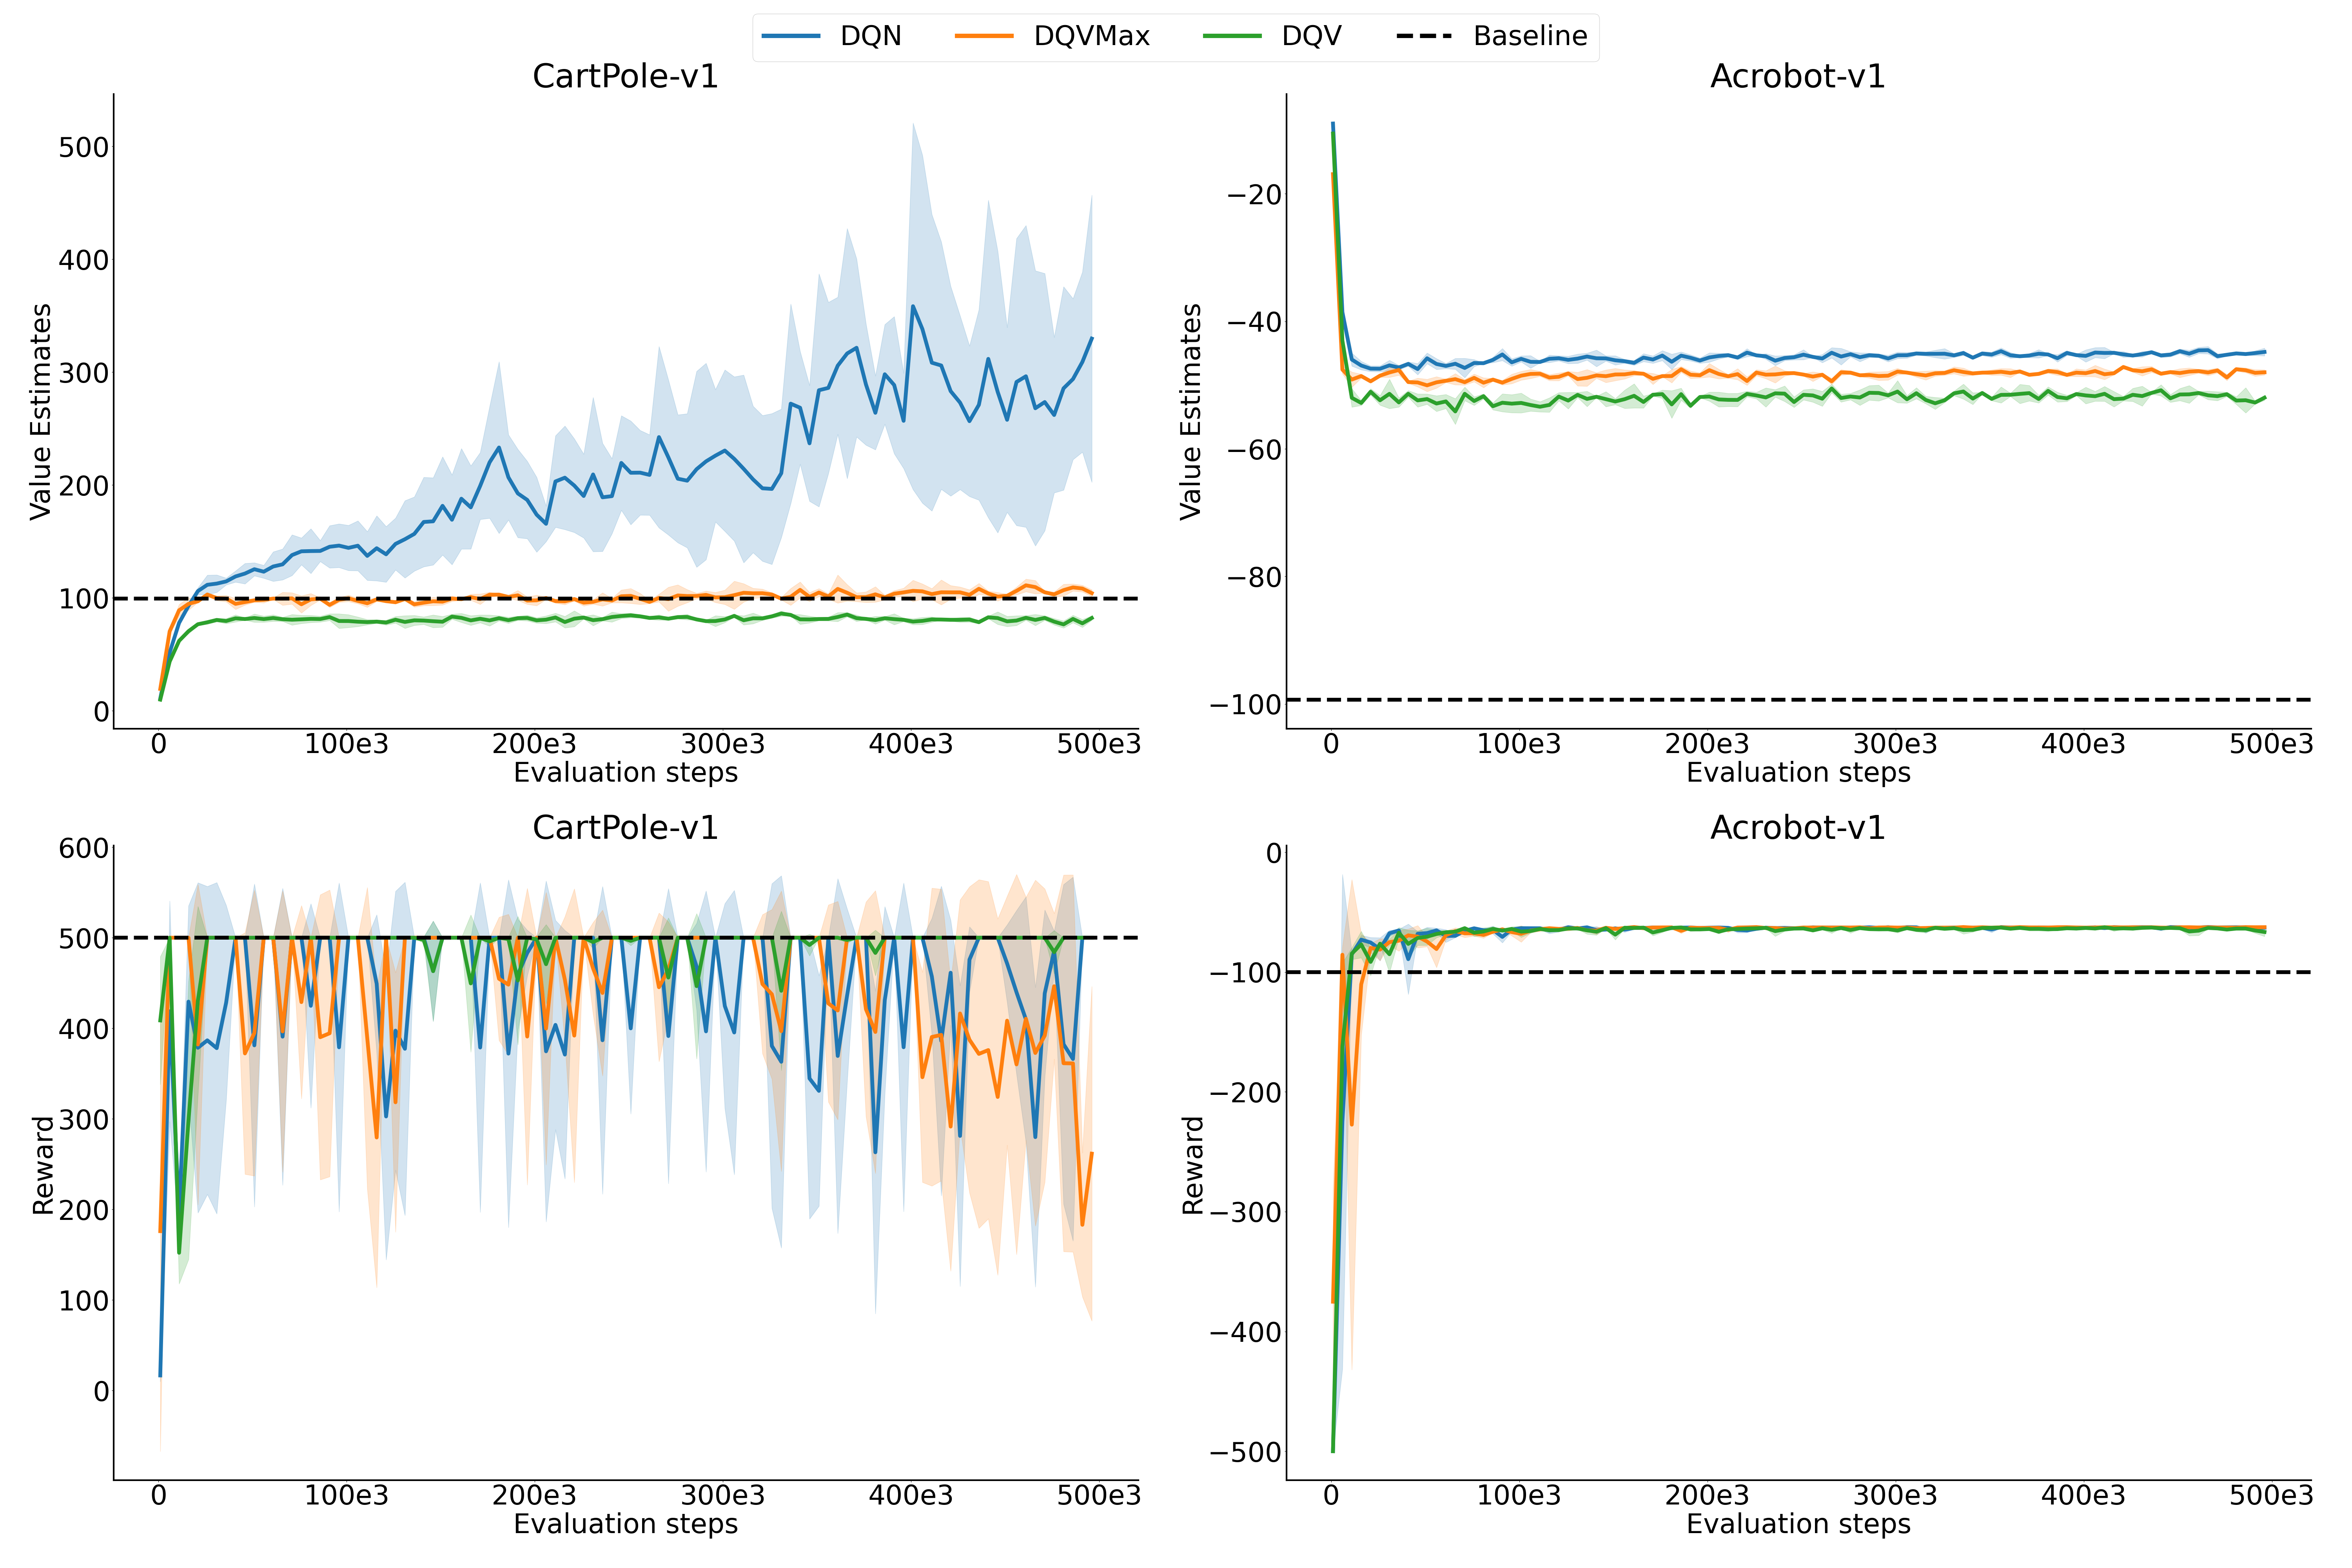
\includegraphics[width=.5\textwidth]{img/dshift_plots_normal.png}
  \caption{The $Q$-value estimates (top row) and actual return curves
    of offline DQN, DQV and DQV-Max at evaluation time. The shaded
    areas are $\pm$ 1 standard deviation from the mean of 3 different
    simulations.}\label{fig:dshift_offline_normal}
\end{figure}

\begin{figure}[!tbp]
  \centering
  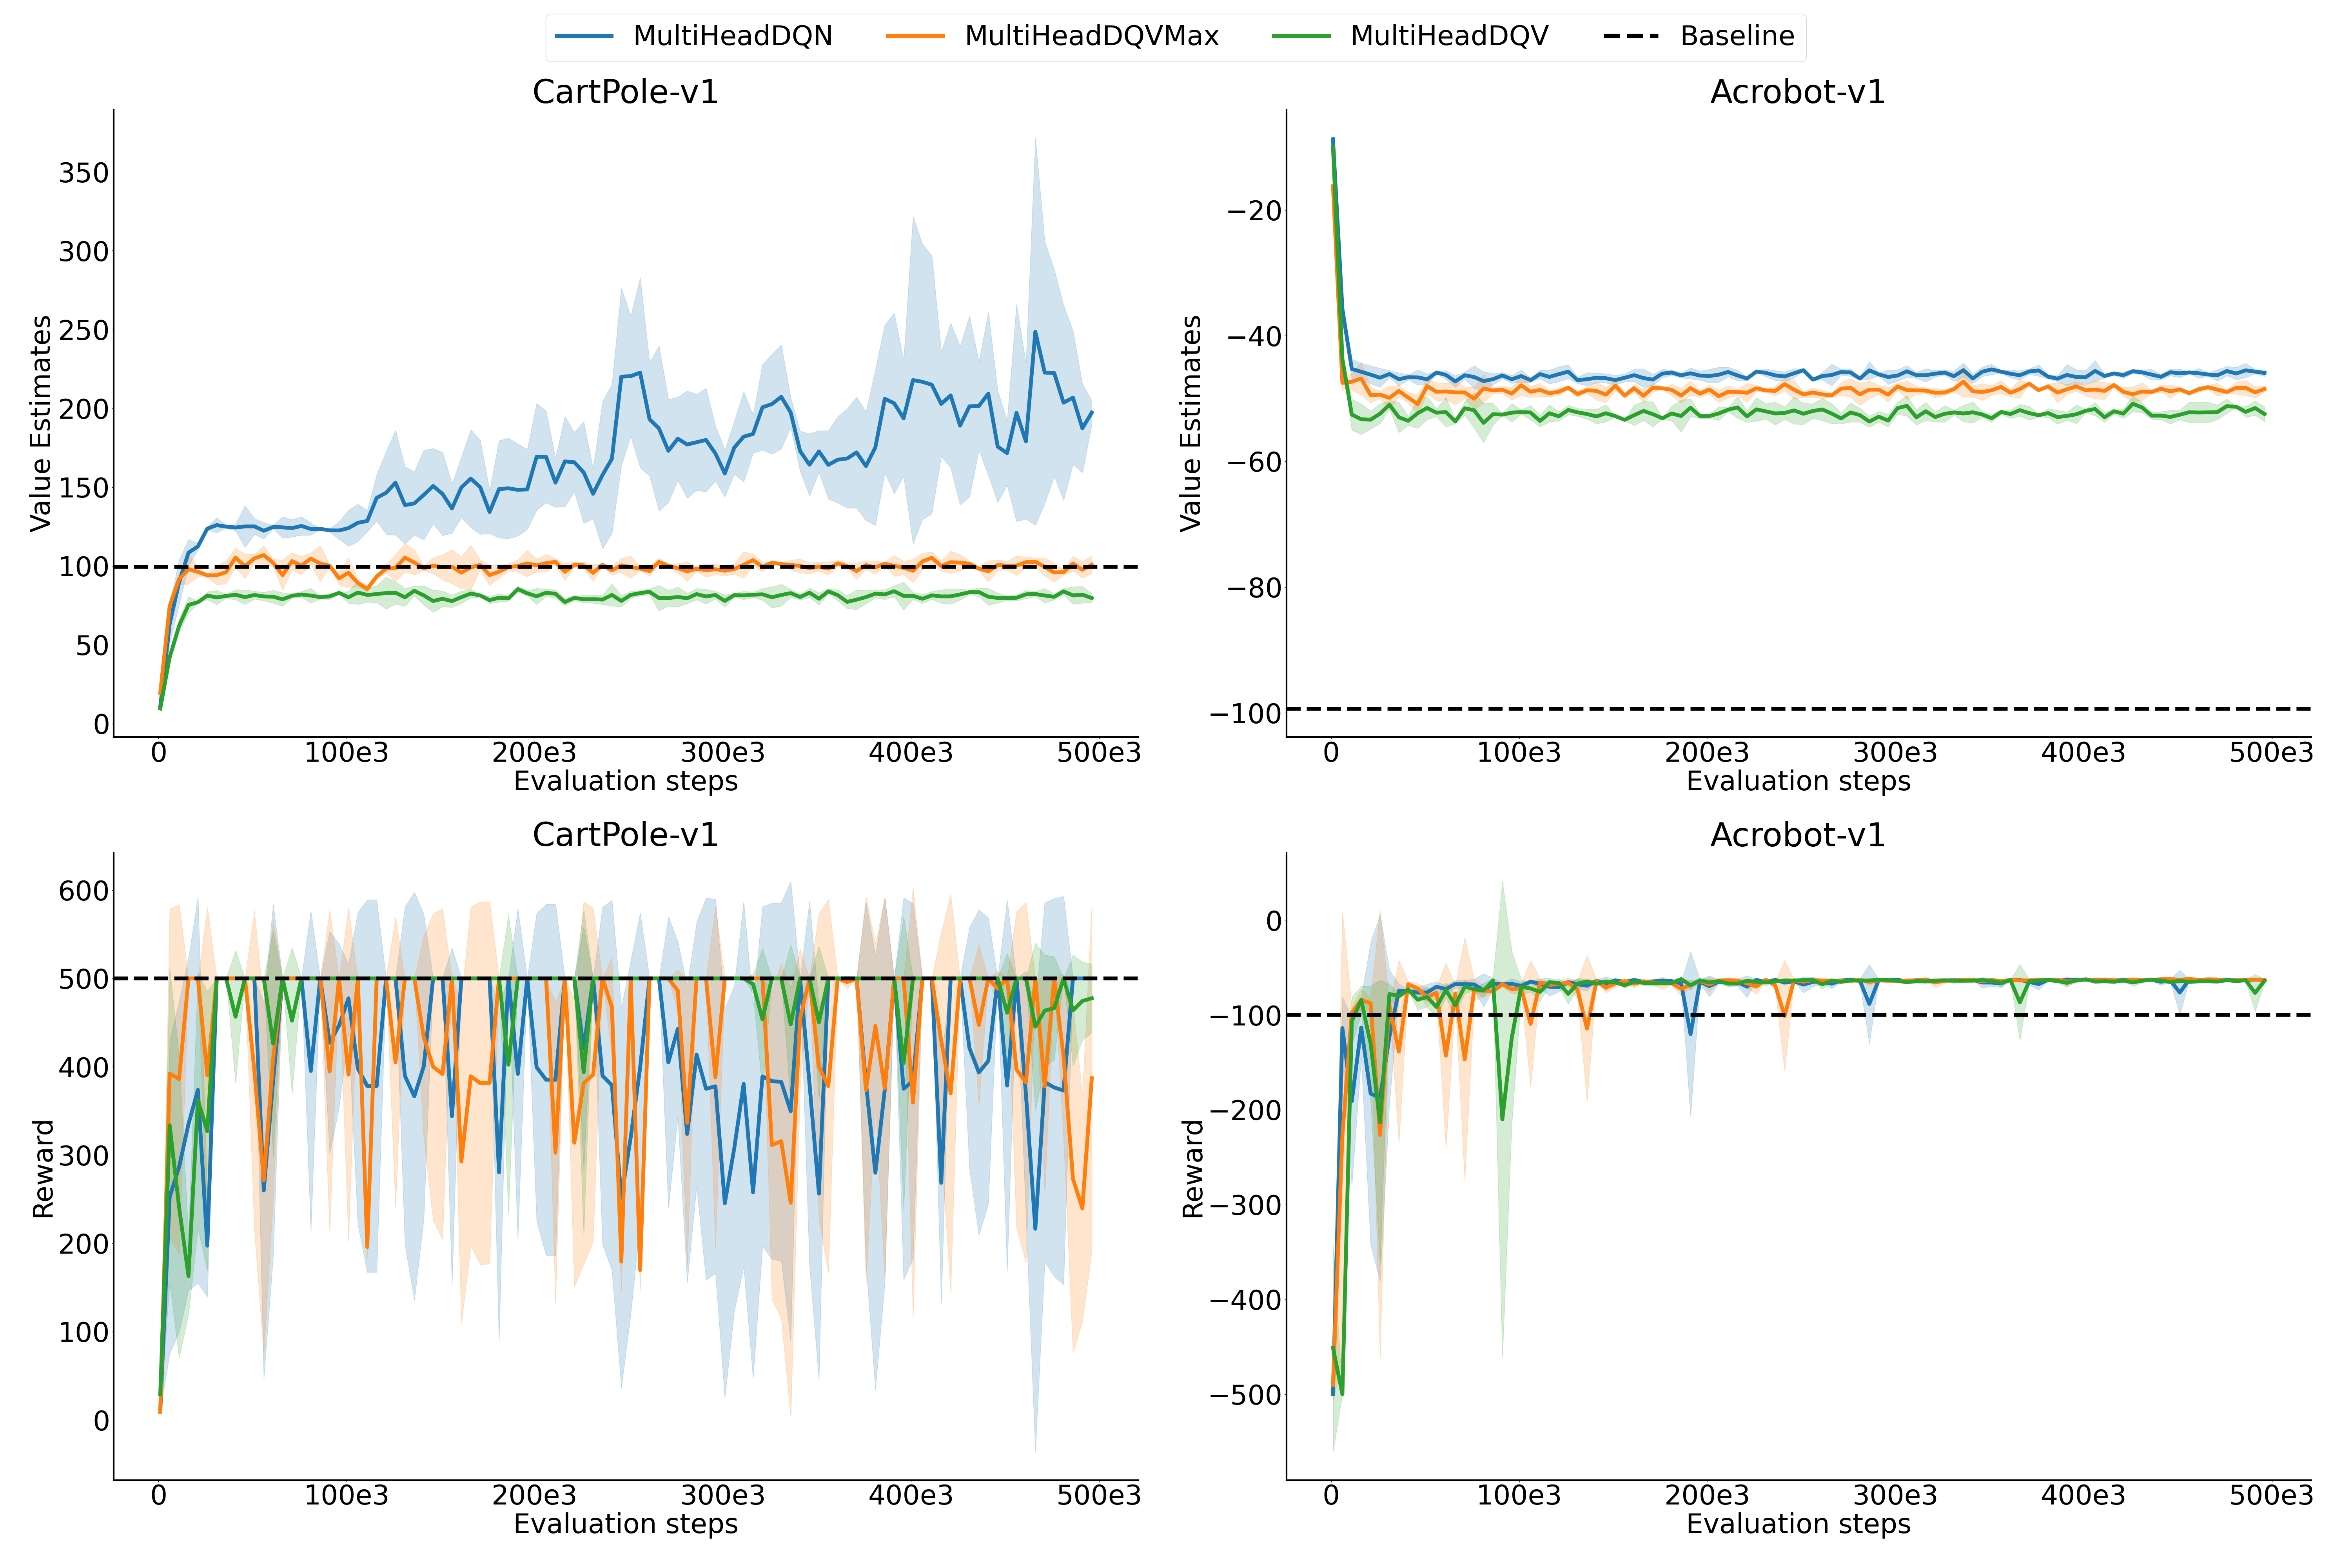
\includegraphics[width=.5\textwidth]{img/dshift_plots_ensembles.png}
  \caption{The $Q$-value estimates (top row) and actual return curves
    of offline DQN, DQV and DQV-Max at evaluation time. The shaded
    areas are $\pm$ 1 standard deviation from the mean of 3 different
    simulations.}\label{fig:dshift_offline_ensembles}
\end{figure}
\section{Conclusion}\label{sec:Conclusion}
% TS: general conclusion: no gains from bare ensemble technique
% implemented as is
The experiments presented in the previous section provide an answer to the
question of whether the DQV algorithmic family benefits from ensemble
techniques when doing offline RL.\ According to the
empirical results, simply re-framing the learning problem of
offline RL to use multiple copies of the same agent is not enough to
prevent the bootstrapping error. Ensembles of function approximators
are a well-known performance boost in machine learning, but it is
crucial to properly exploit the additional information they provide
compared to a single learner. If this point is not correctly
addressed, the possible uncertainty estimation gains are overlooked,
and such information is critical for an offline RL agent.

% LIMITATIONS
% TS: one limitation is the DQV family, which is too strong and
% already acts where the bootstrapping error takes place, so they are
% inherently wrong to use with naive ensembles
When testing whether the simple ensemble technique of Ensemble-DQN can
be generalized to other algorithms, translating it to DQV and DQV-Max
becomes a limitation of this study. In fact, as already mentioned,
these algorithms disentangle \textit{selection} -- the choice of the
regression targets for the state or state-action value function --
from \textit{evaluation} -- the estimation of a state or
state-action pair's value. This is one important factor in the infamous
\textit{deadly triad} of off-policy RL
\citep{sutton2018reinforcement}, and the main focus of this research
under the form of bootstrapping error. Where such decoupling is absent,
as in the DQN algorithm, using a simple ensemble was in fact enough to
observe gains in terms of variance reduction, which is directly
related to the overestimation bias \citep{anschel2017averaged} and
results from misaligned value estimates -- also known as bootstrapping
errors. This was the case for the experiments with offline
Ensemble-DQN on the \texttt{CartPole-v1} environment. When it comes to
the DQV algorithmic family and controlling the bootstrapping error
with ensembles, these algorithms' strength thus becomes an
architectural weakness for the proposed experiments. In fact, base DQV
and DQVMax show a robust performance in the offline setting that is
unaffected by the addition of more heads to estimate uncertainty.
By using a different function to form the
TD-targets than to evaluate current states, these algorithms already
take significant steps to prevent the bootstrapping error, which
makes them unfit candidates for the simple ensemble strategy of
Ensemble-DQN.\

% TS: another limitation is the naive ensemble technique used, which is
% a simple average over heads for both Q(s',a') and Q(s,a) and trains
% everyone on the same loss
Another limitation is the naive ensemble technique employed throughout
the experiments adapted from Ensemble-DQN.\ Given the empirical
results, it is not sufficient to increase the number of prediction
heads in DQV and DQV-Max, apply standard value-based regression
methods (i.e.\ temporal difference learning) individually on each,
then train
every head on the average of the ensemble total loss. As
previously stated, the former are two strong off-policy algorithm; yet
for
offline RL they could still benefit from the uncertainty estimated by
an ensemble of $Q$ or $V$ functions, if this information is properly
integrated in their learning formulation. The simple averaging technique
implemented in this research does not fully exploit the uncertainty
information provided by the ensembles of $Q$ and $V$ functions. It
would be interesting to see what happens when conservative estimates
are formed in the face of uncertainty, for example, by down-scaling
the TD-targets by the variance of the ensemble predicted $Q$-values as
discussed in \citet{levine2020offline}.

% FUTURE RESEARCH
% TS: cool to see if dqv and dqvmax are strong alone with less and/or
% worse online training data
For future work with a setup similar to this research, different lines
of experimentation are possible. For example, the size and diversity
of the offline dataset $\mathcal{B}$ collected by $\pi_{\beta}$ could
be manipulated to asses the generalization capabilities of offline DQV
and DQV-Max. As seen in some of the experiments for the REM agent
\citep{agarwal2020optimistic}, one could reduce the size of the
dataset
$\mathcal{B}$ to find the minimum amount of trajectories needed to
obtain an acceptable performance. Alternatively, offline DQV and
DQV-Max could be
given only expert or quasi-random data, thus decreasing $\mathcal{B}$'s
diversity. The offline agents in this research learned on the full set
of policies encountered during online training of $\pi_{\textrm{DQN}}$; this
was done in order to establish a safe baseline in lieu of the
importance of training datasets' diverse composition highlighted by
the REM results.
Learning on data produced by a small number of policies or by
highly suboptimal ones matters for offline DQV and DQV-Max because it
resembles what is available from many settings in the real world,
where behavioral data are collected by a handful of static policies --
or even a single one.

% TS: move uncertainty estimation out of the single algorithm scope,
% and use it when combining different conceptually different learners;
% ultimately, try voting ensembles, e.g. DQV and DQV-Max
Finally, regarding uncertainty estimation in offline RL, the ensemble
component could be extracted from the single algorithm scope and
applied to different learners. This means having a multitude of agents
(e.g.\ both DQV and DQV-Max) learn and collaborate on the same
problem, implementing a voting procedure to decide, for example, on
the TD-targets for the whole ensemble. The same information
relating to uncertainty estimation purposes available from individual
heads in the current setup could then come from different RL
algorithms that inform the ensemble decisions. Voting ensembles are a
well-defined concepts in machine learning, and in the case of DQV and
DQV-Max it could be of interest to assess if the relative strength of
each agent taken individually -- lower variance for the first
on-policy algorithm, greater learning generality for the second
off-policy one -- can be combined in a meaningful way on the offline
RL setting.


\bibliographystyle{apacite}
\bibliography{bibliography}

\clearpage

\begin{appendices}
  \section{Appendix}
  Following the practice from \citet{DBLP:journals/corr/abs-1709-06560}
  and \citet{https://doi.org/10.48550/arxiv.1904.06979}, Welch's
  \textit{t}-test was used to test whether each ensemble variant of the
  analyzed algorithms performed worse than its respective base version
  in terms of the defined response metrics. Significant results are
  highlighted in Table~\ref{table:center_results}.
  For the Ensemble-DQV-Max ablations experiment, a Kruskal-Wallis H-test
  was used to compare the former agent to its ablated variants.
  Both test were performed with the corresponding routines from the
  \texttt{SciPy} Python package \citep{2020SciPy-NMeth}.

  \subsection{Additional plots}\label{sec:appendix_figs}
\begin{figure}[H]
  \centering
  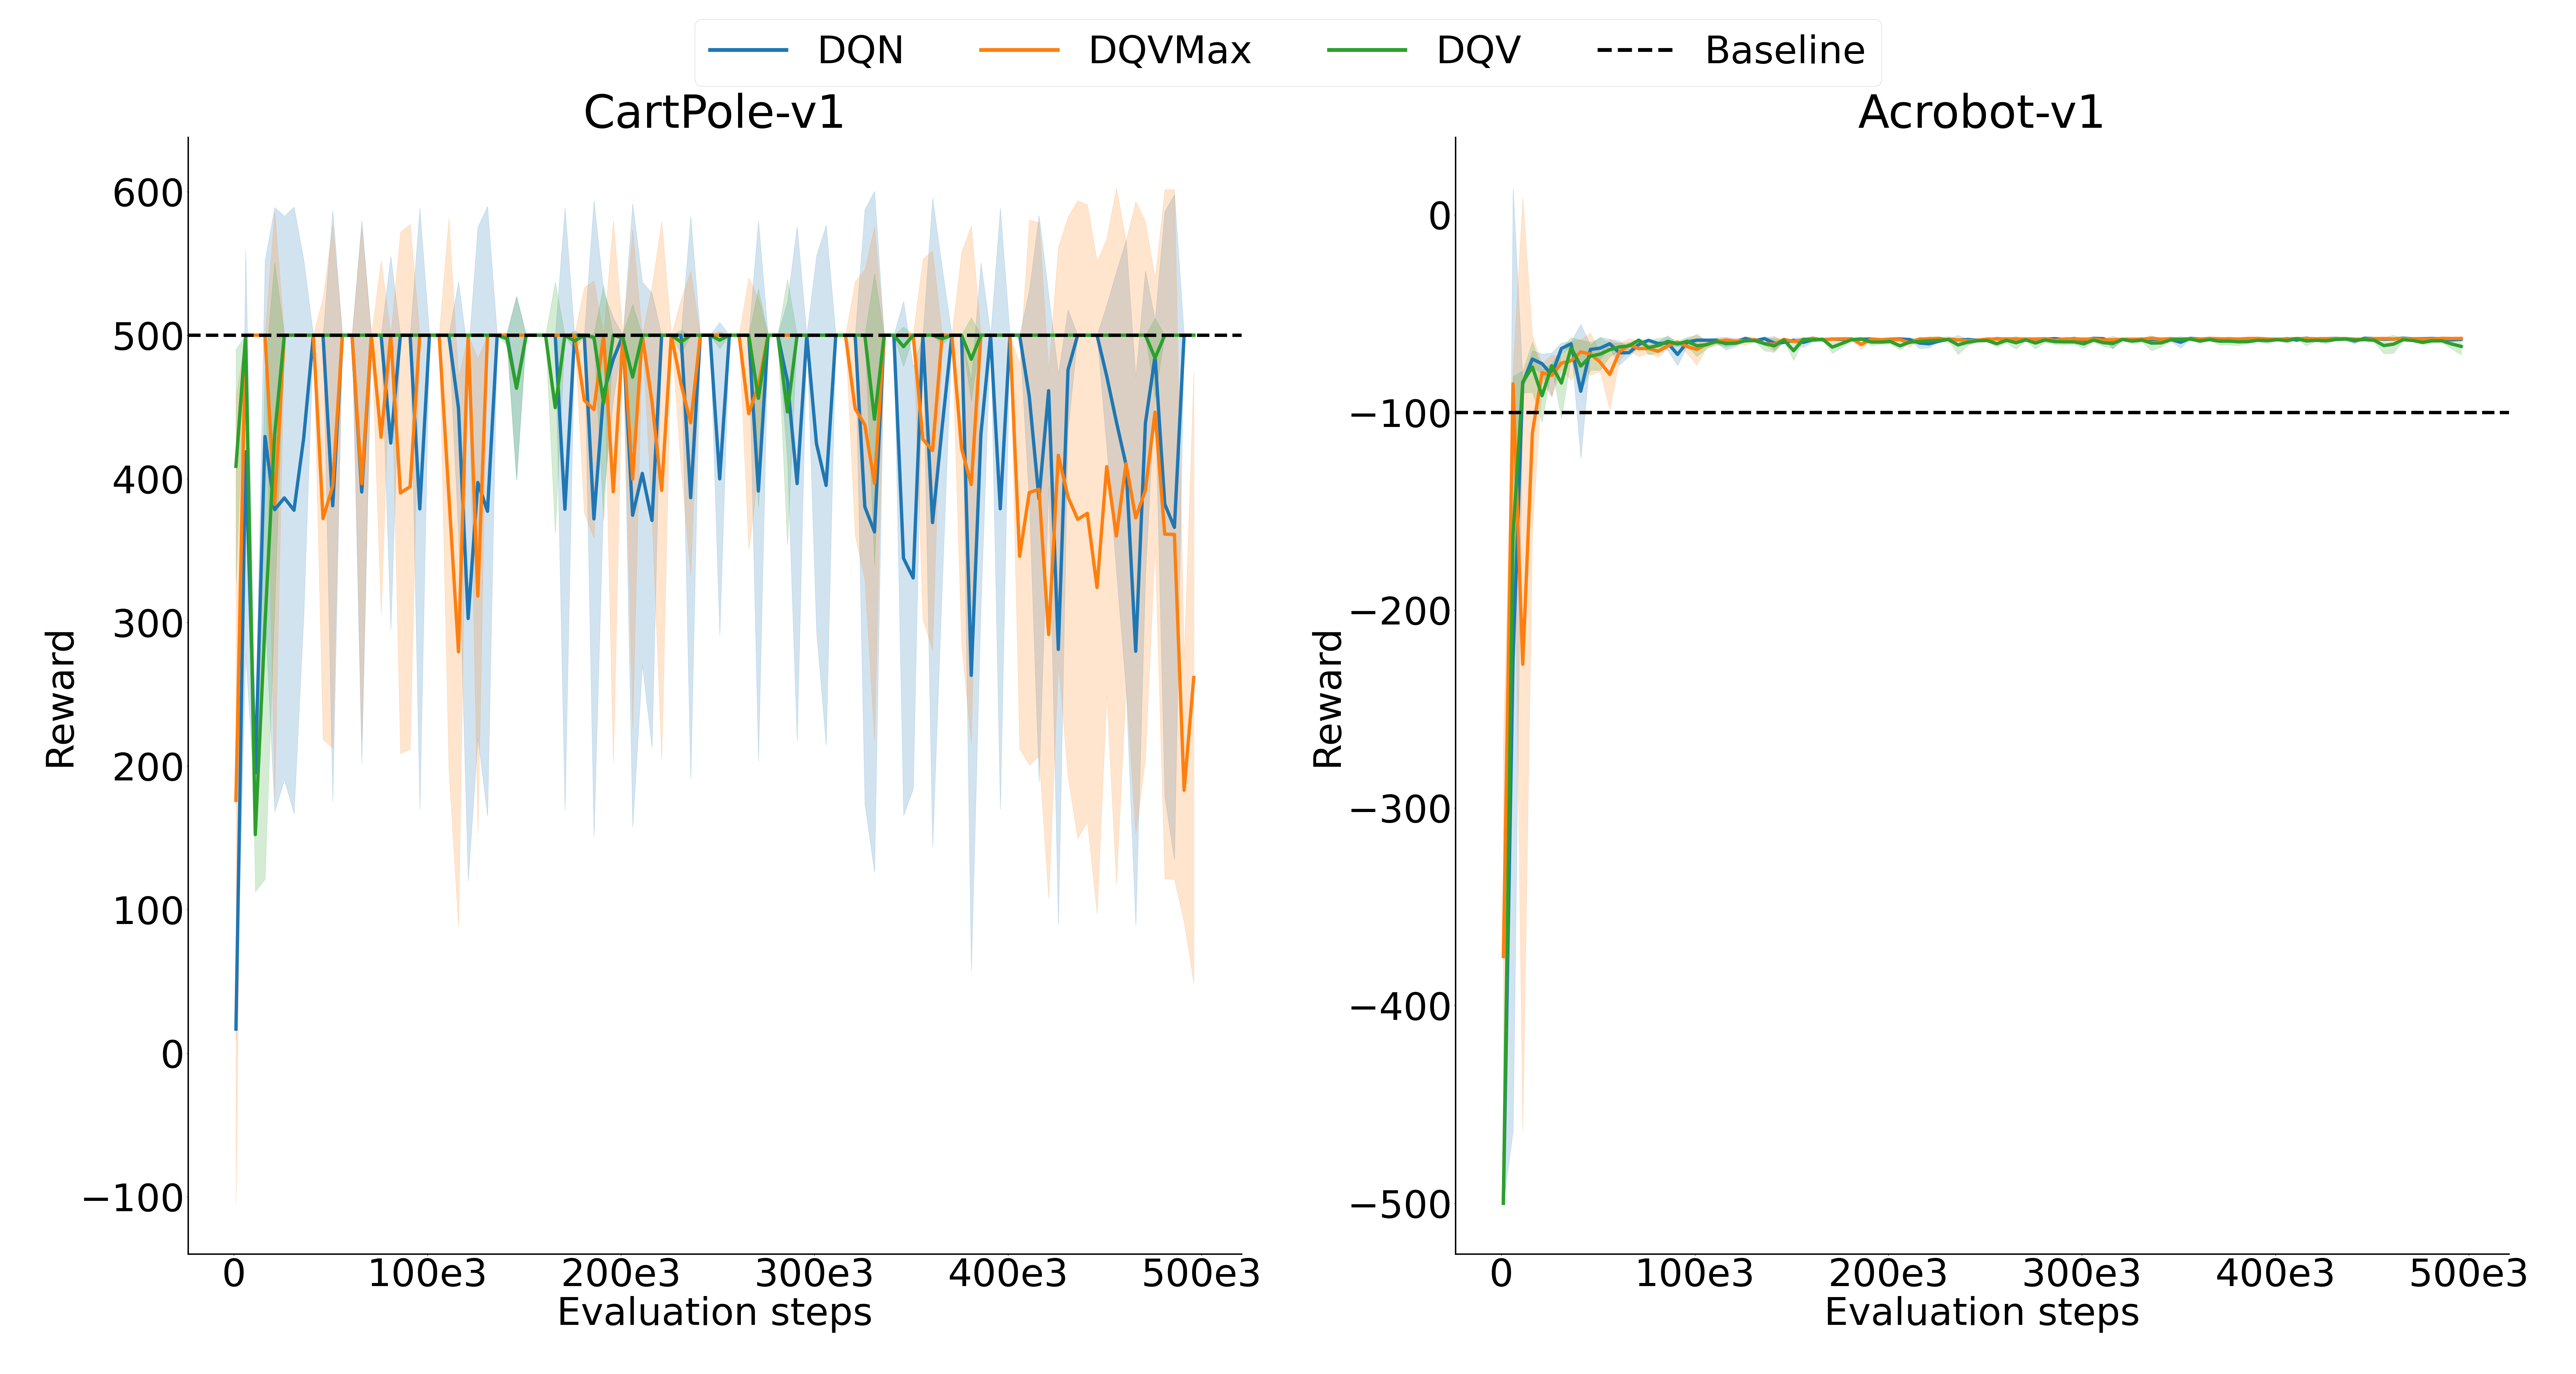
\includegraphics[width=.5\textwidth]{img/dshift_plots_rwd.png}
  \caption{Evaluation time reward signal for offline DQN, DQV and
    DQV-Max, averaged over 3 runs}\label{fig:dshift_rwd}
\end{figure}

\begin{figure}[H]
  \centering
  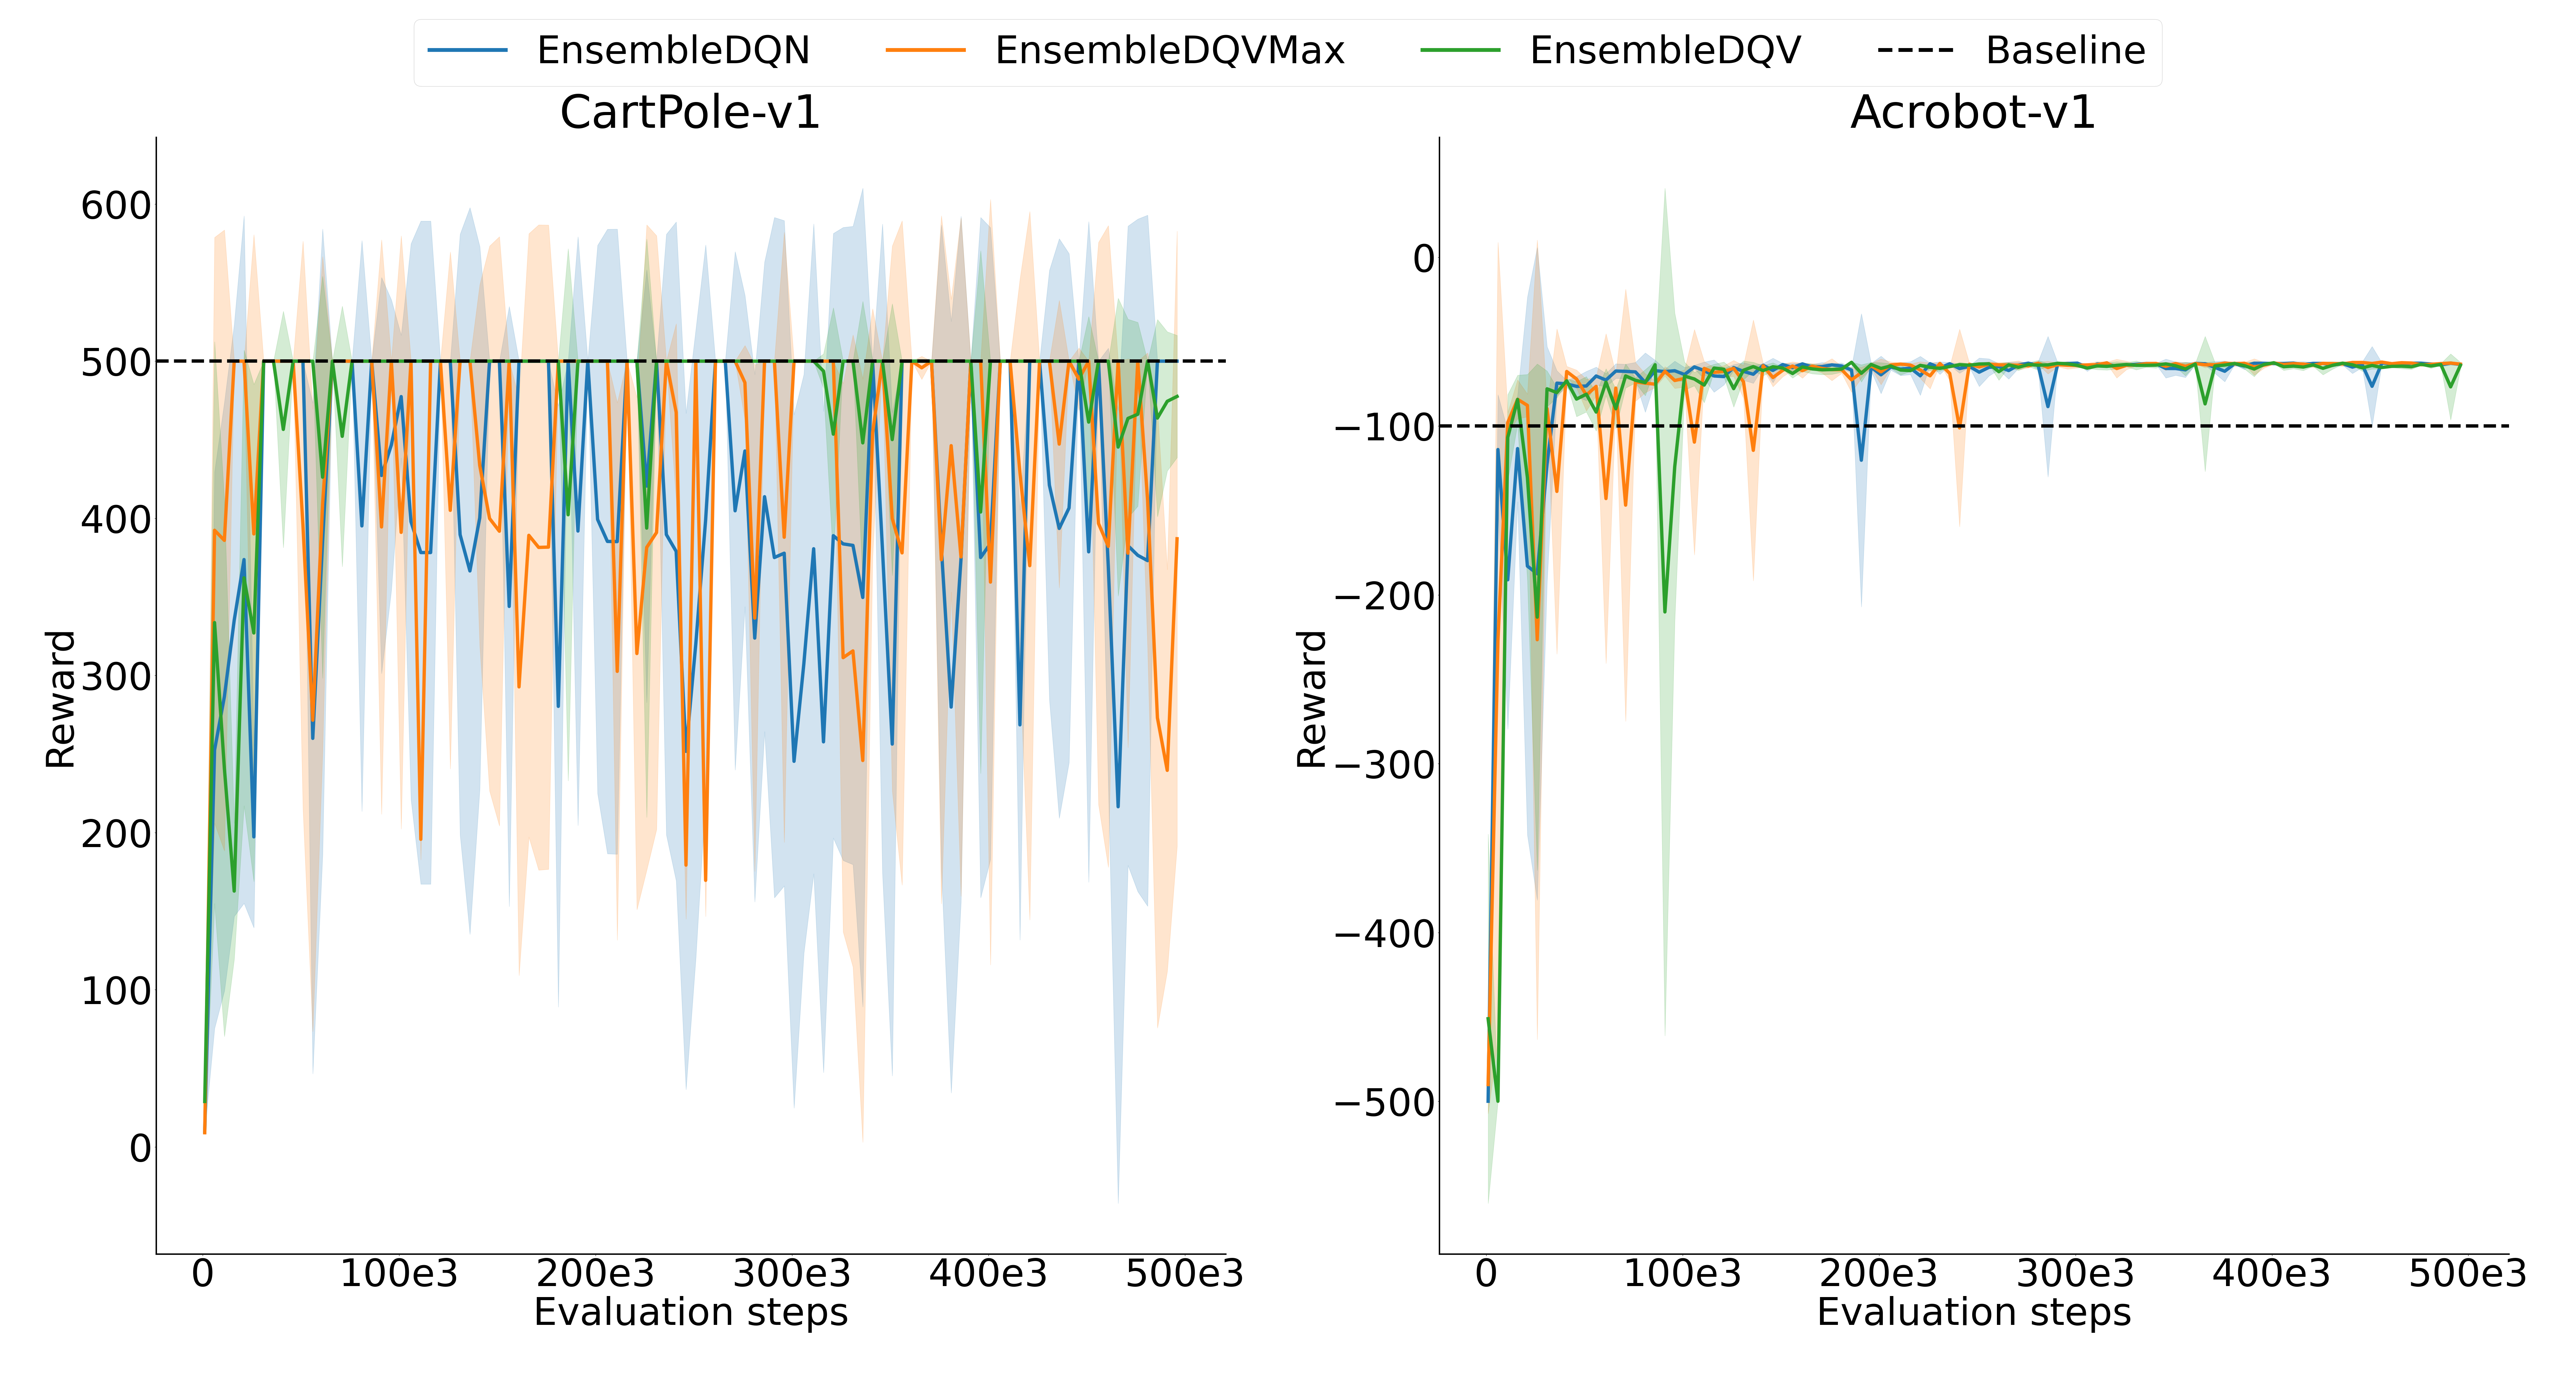
\includegraphics[width=.5\textwidth]{img/dshift_plots_ensembles_rwd.png}
  \caption{Evaluation time reward signal for the ensemble variants of
    offline DQN, DQV and DQV-Max, averaged over 3
    runs}\label{fig:dshift_ensemble_rwd}
\end{figure}

\begin{figure}[H]
  \centering
  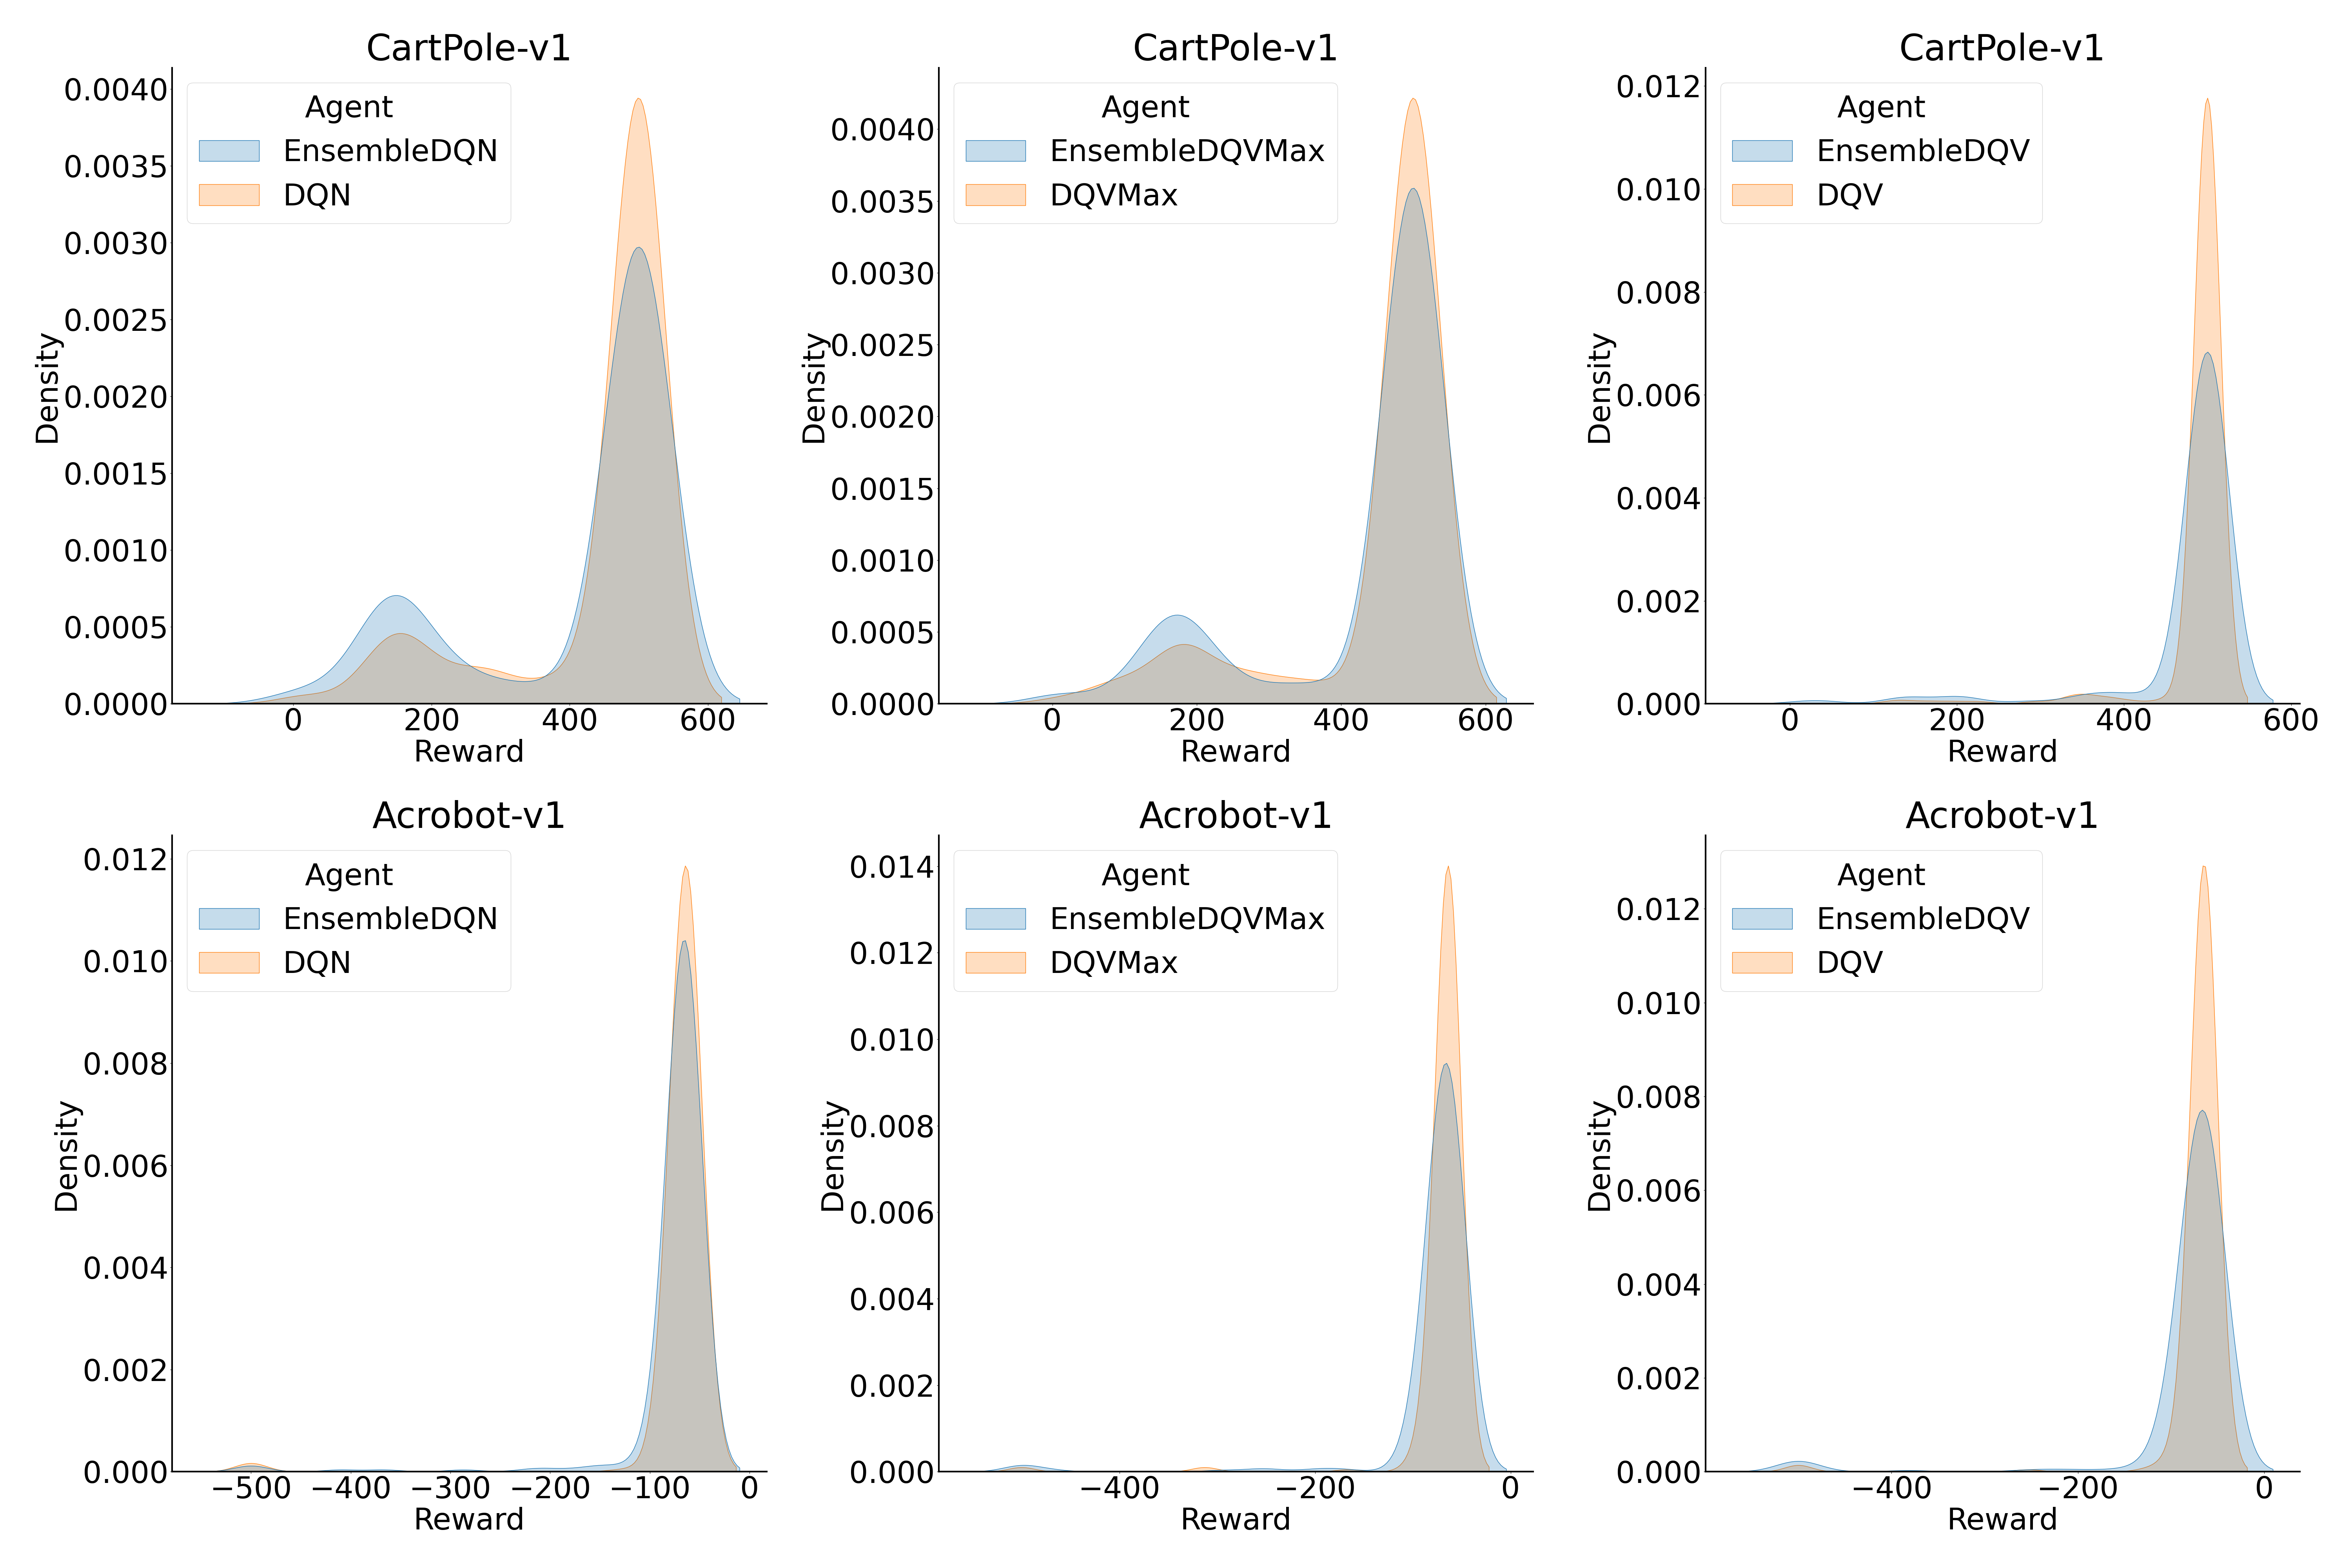
\includegraphics[width=.5\textwidth]{img/all_rwd_dist.png}
  \caption{Distribution of rewards: each offline agent is compared
    against its ensemble variant}\label{fig:rwd_dist}
\end{figure}

\begin{figure}[H]
  \centering
  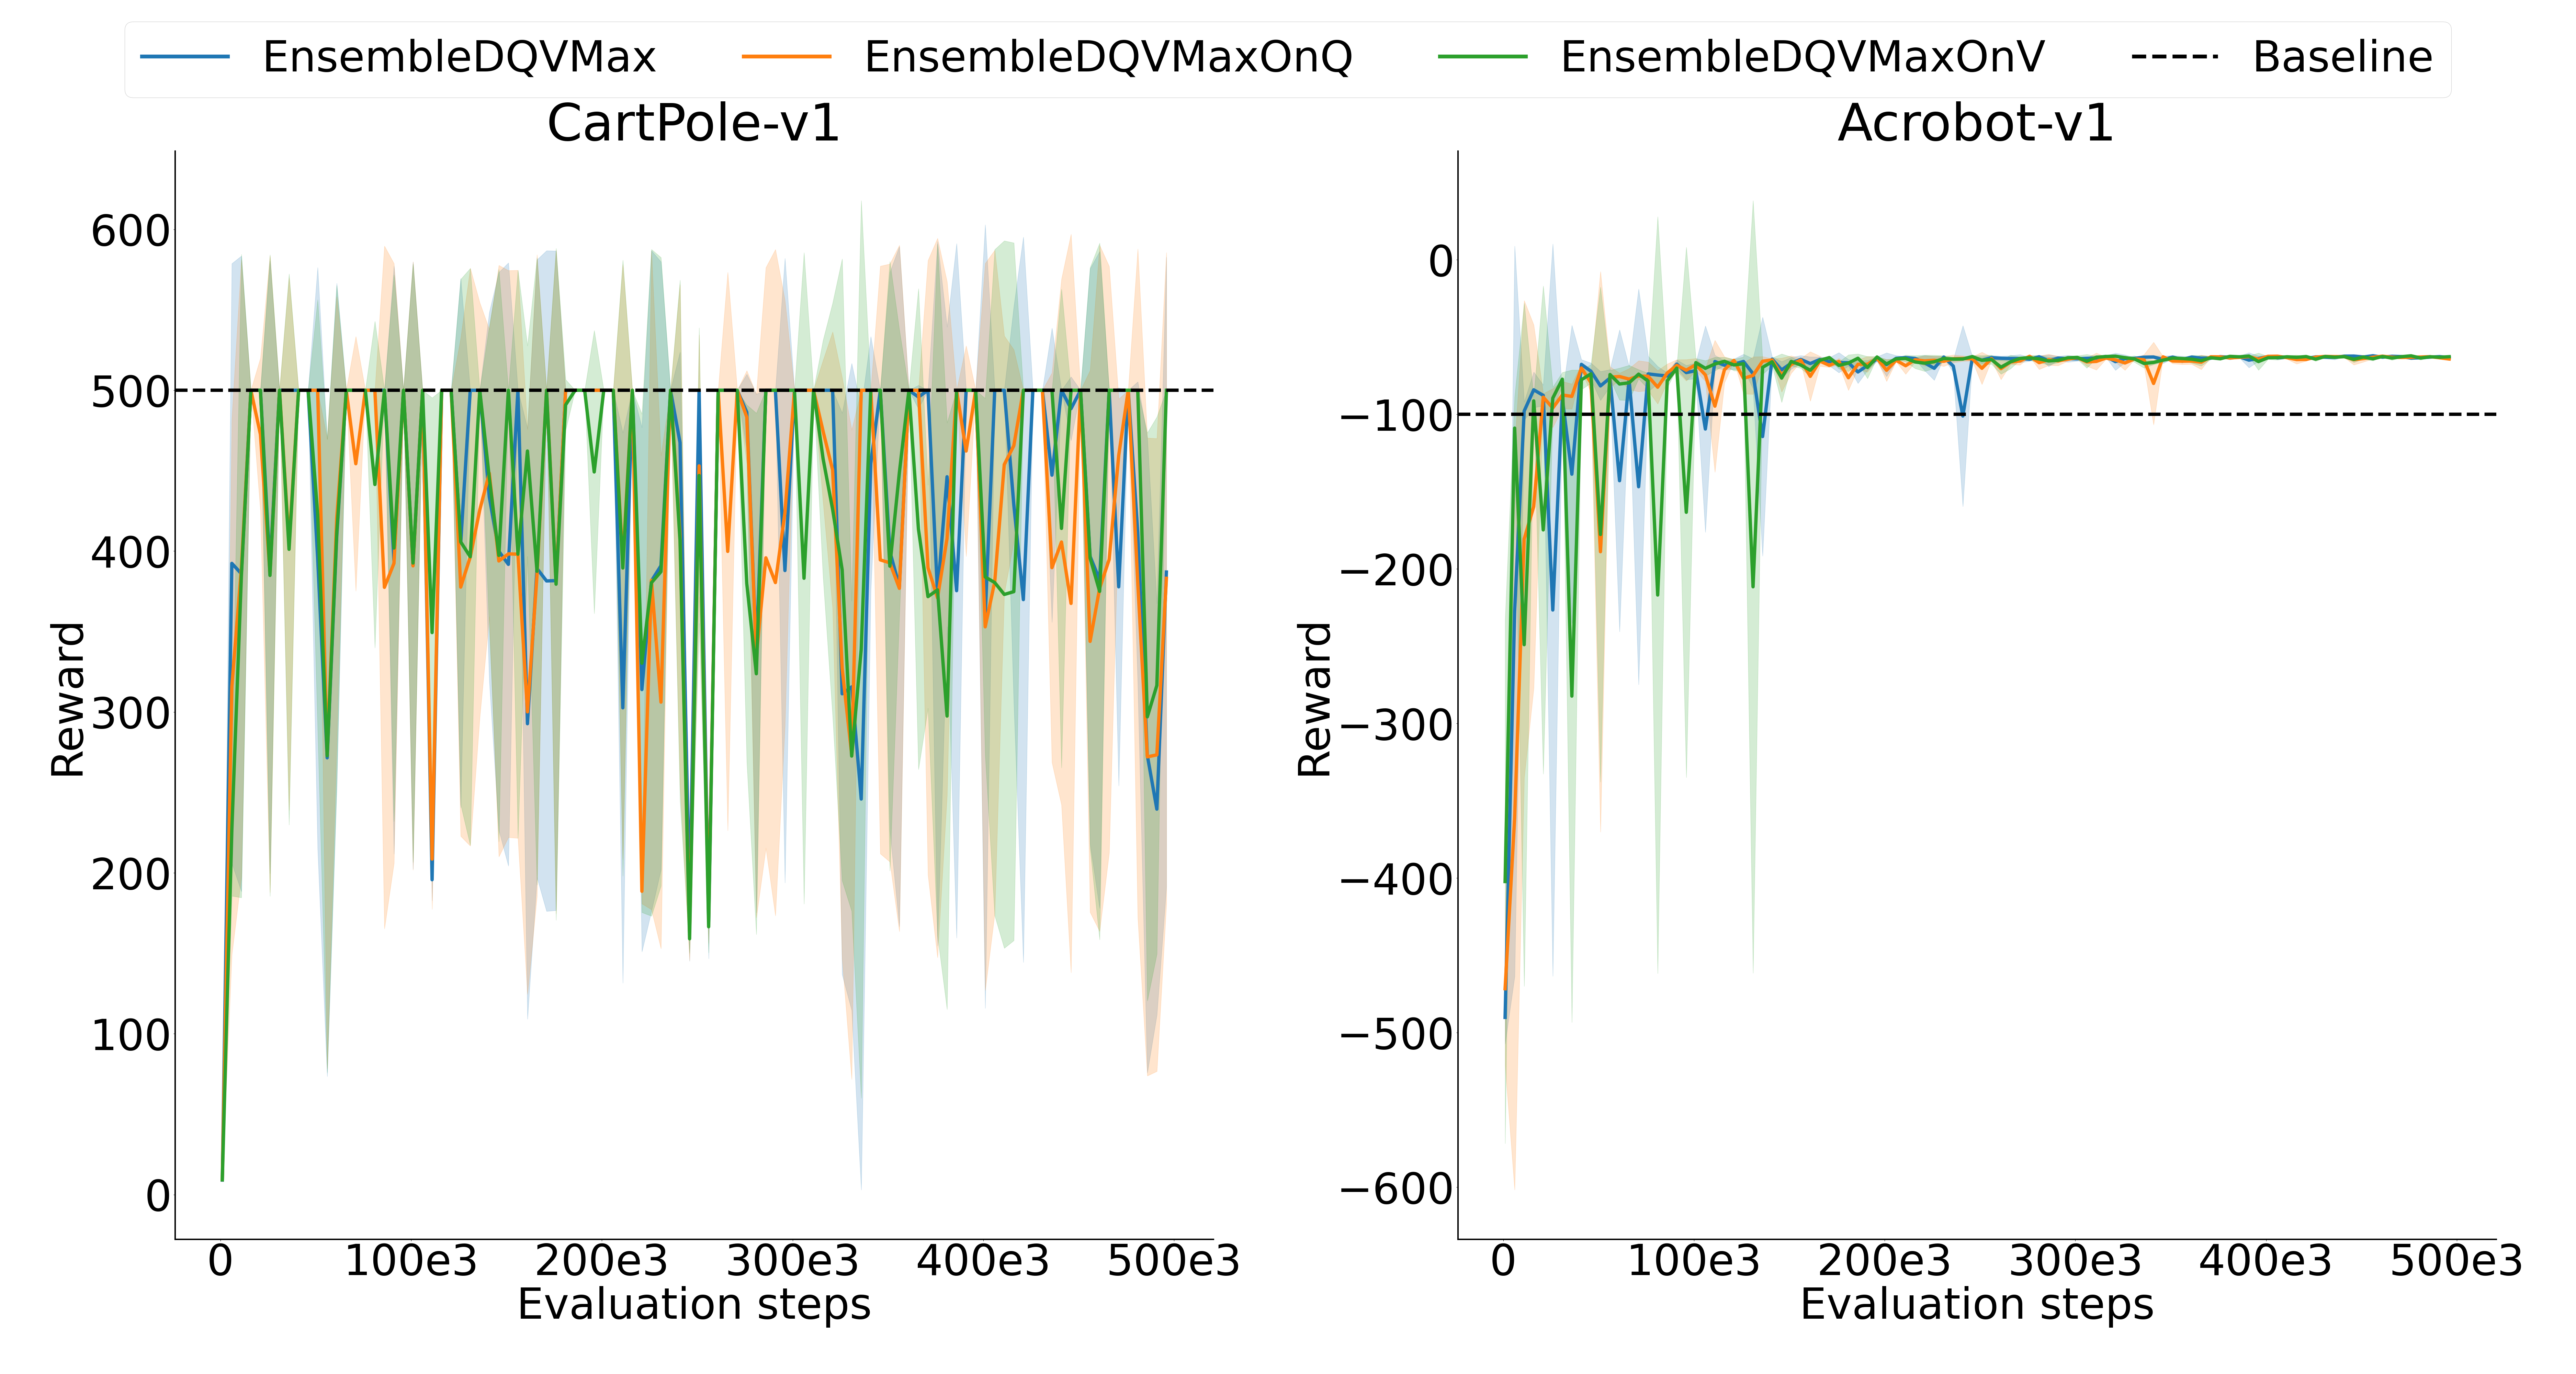
\includegraphics[width=.5\textwidth]{img/dshift_plots_ablation_rwd.png}
  \caption{Ensemble-DQV-Max reward signals for the ablations
    experiment, averaged over 3 runs}\label{fig:dshift_rwd_ablation}
\end{figure}

\begin{figure}[H]
  \centering
  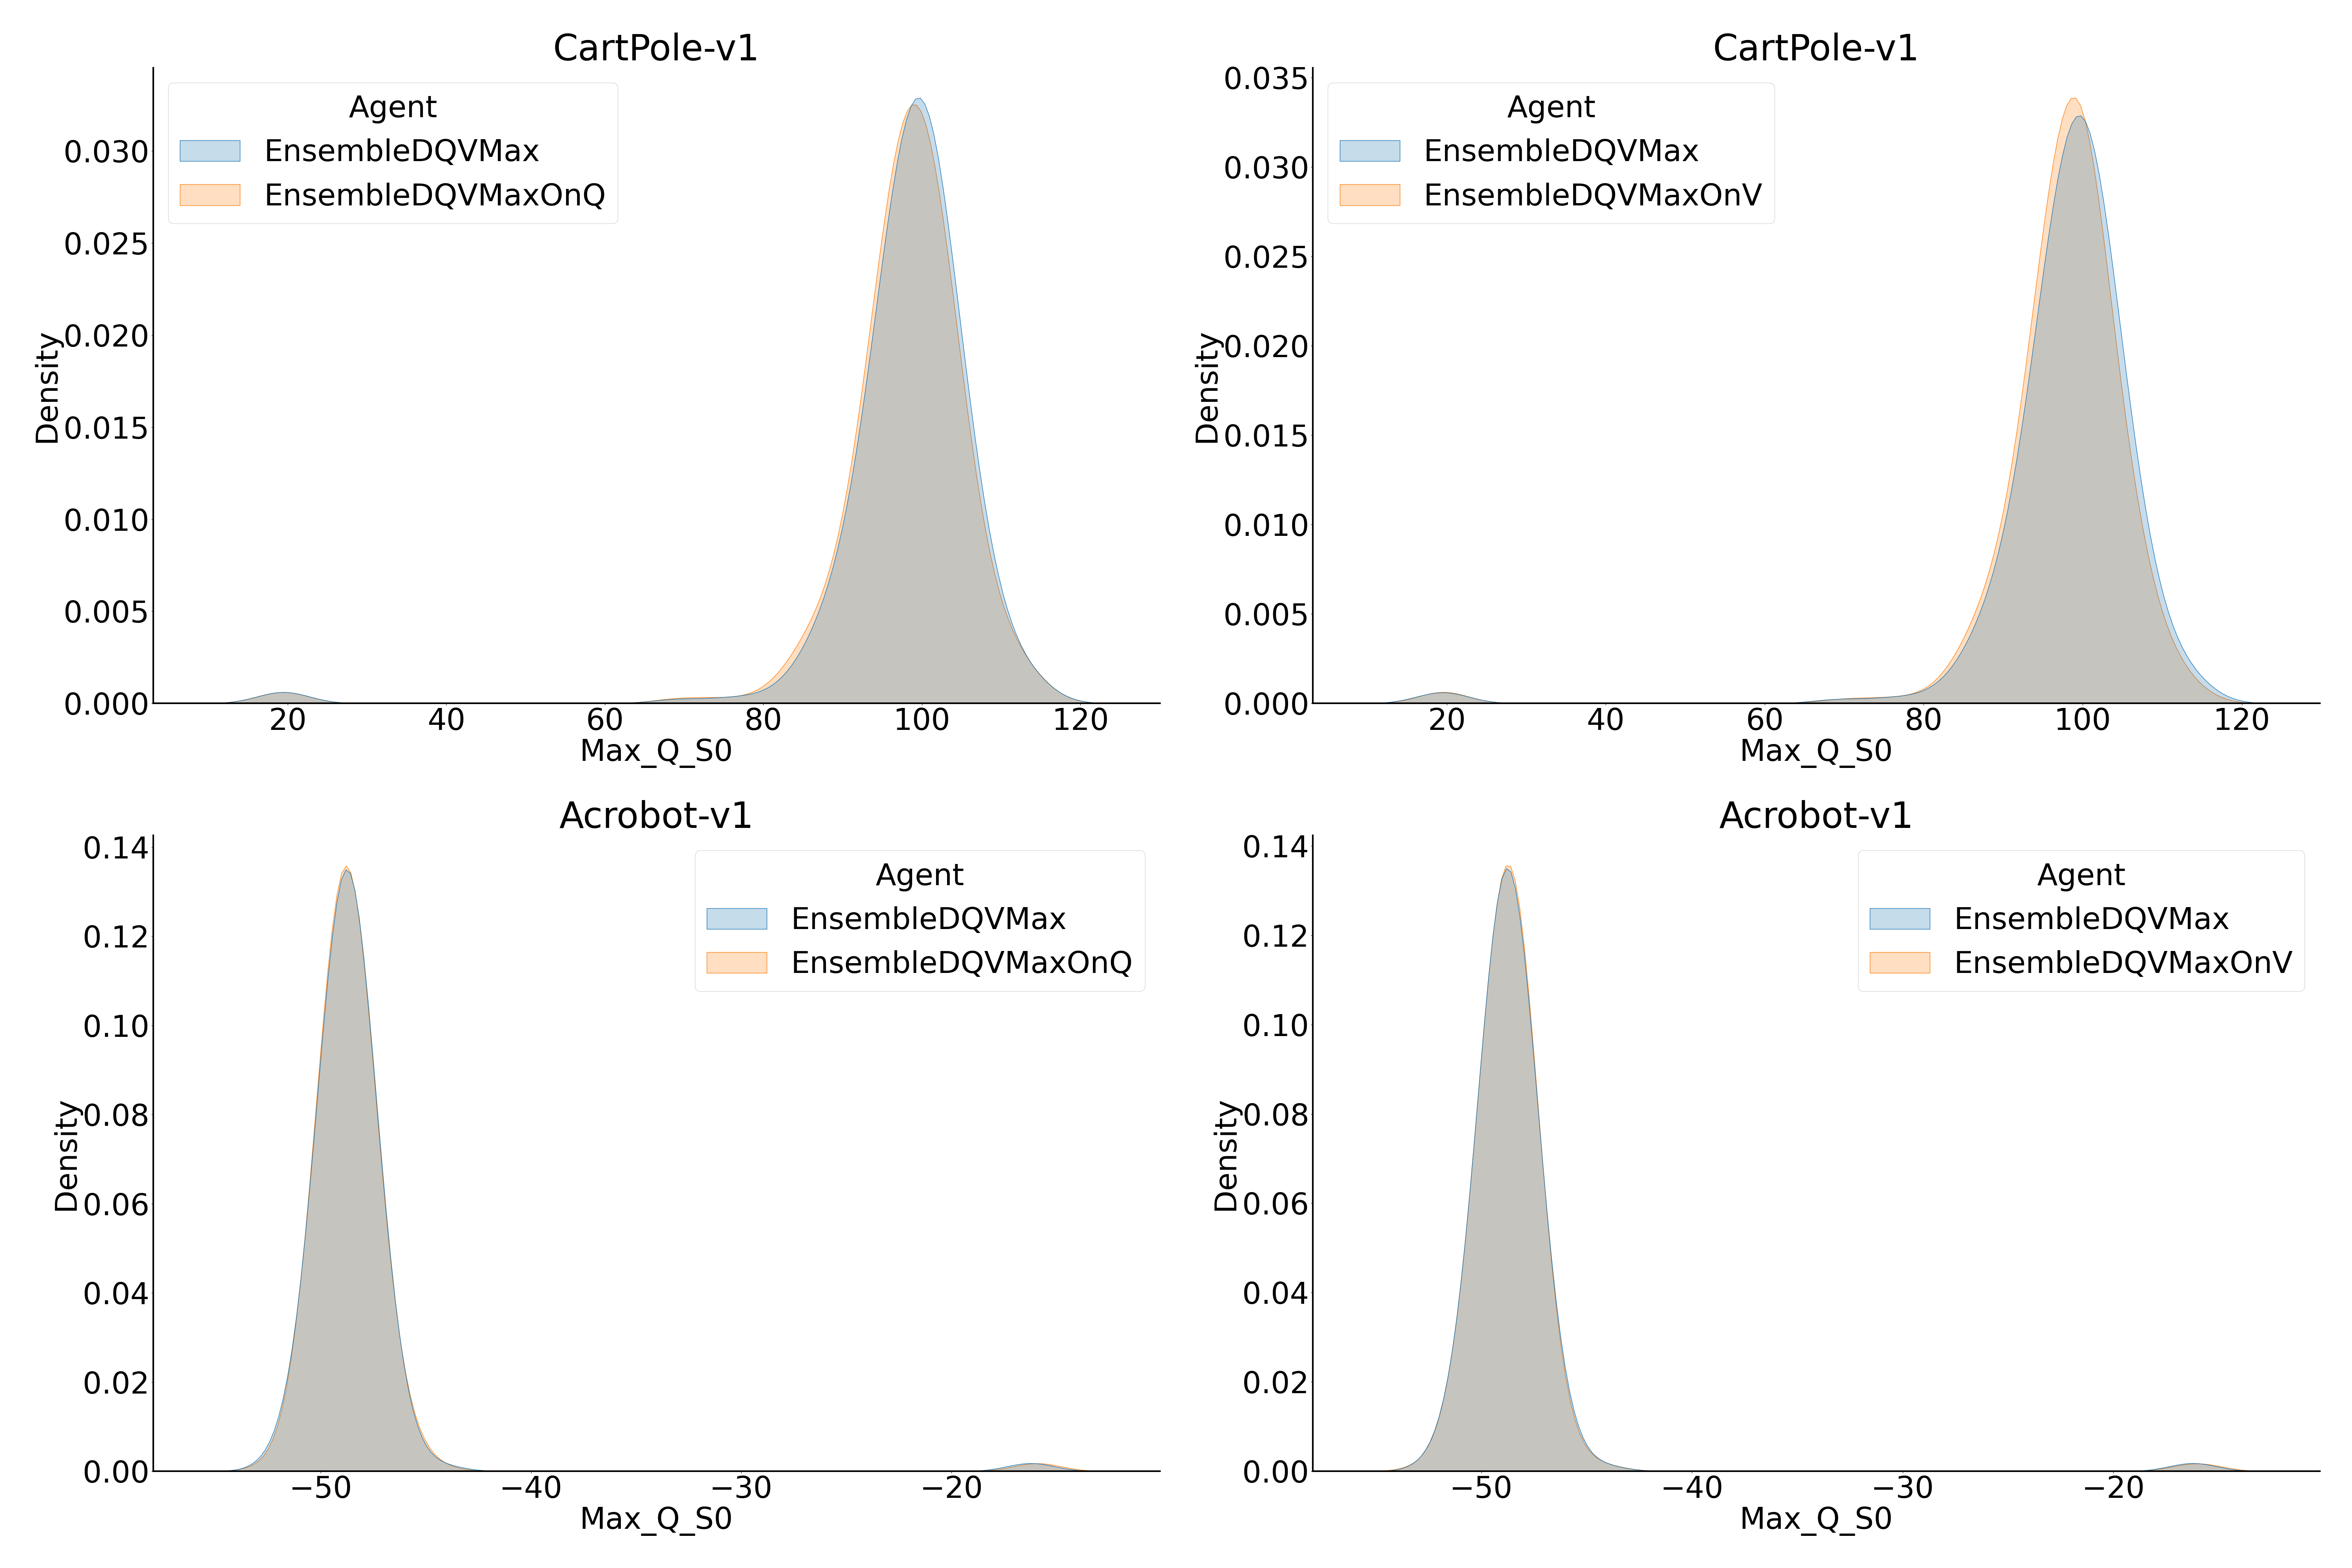
\includegraphics[width=.5\textwidth]{img/dqvmax_abl_qv_dist.png}
  \caption{Distribution of maximum $Q$-values for $s_0$ for
    Ensemble-DQV-Max compared against its
    ablations}\label{fig:dqvmax_abl_qv_dist}
\end{figure}

\begin{figure}[H]
  \centering
  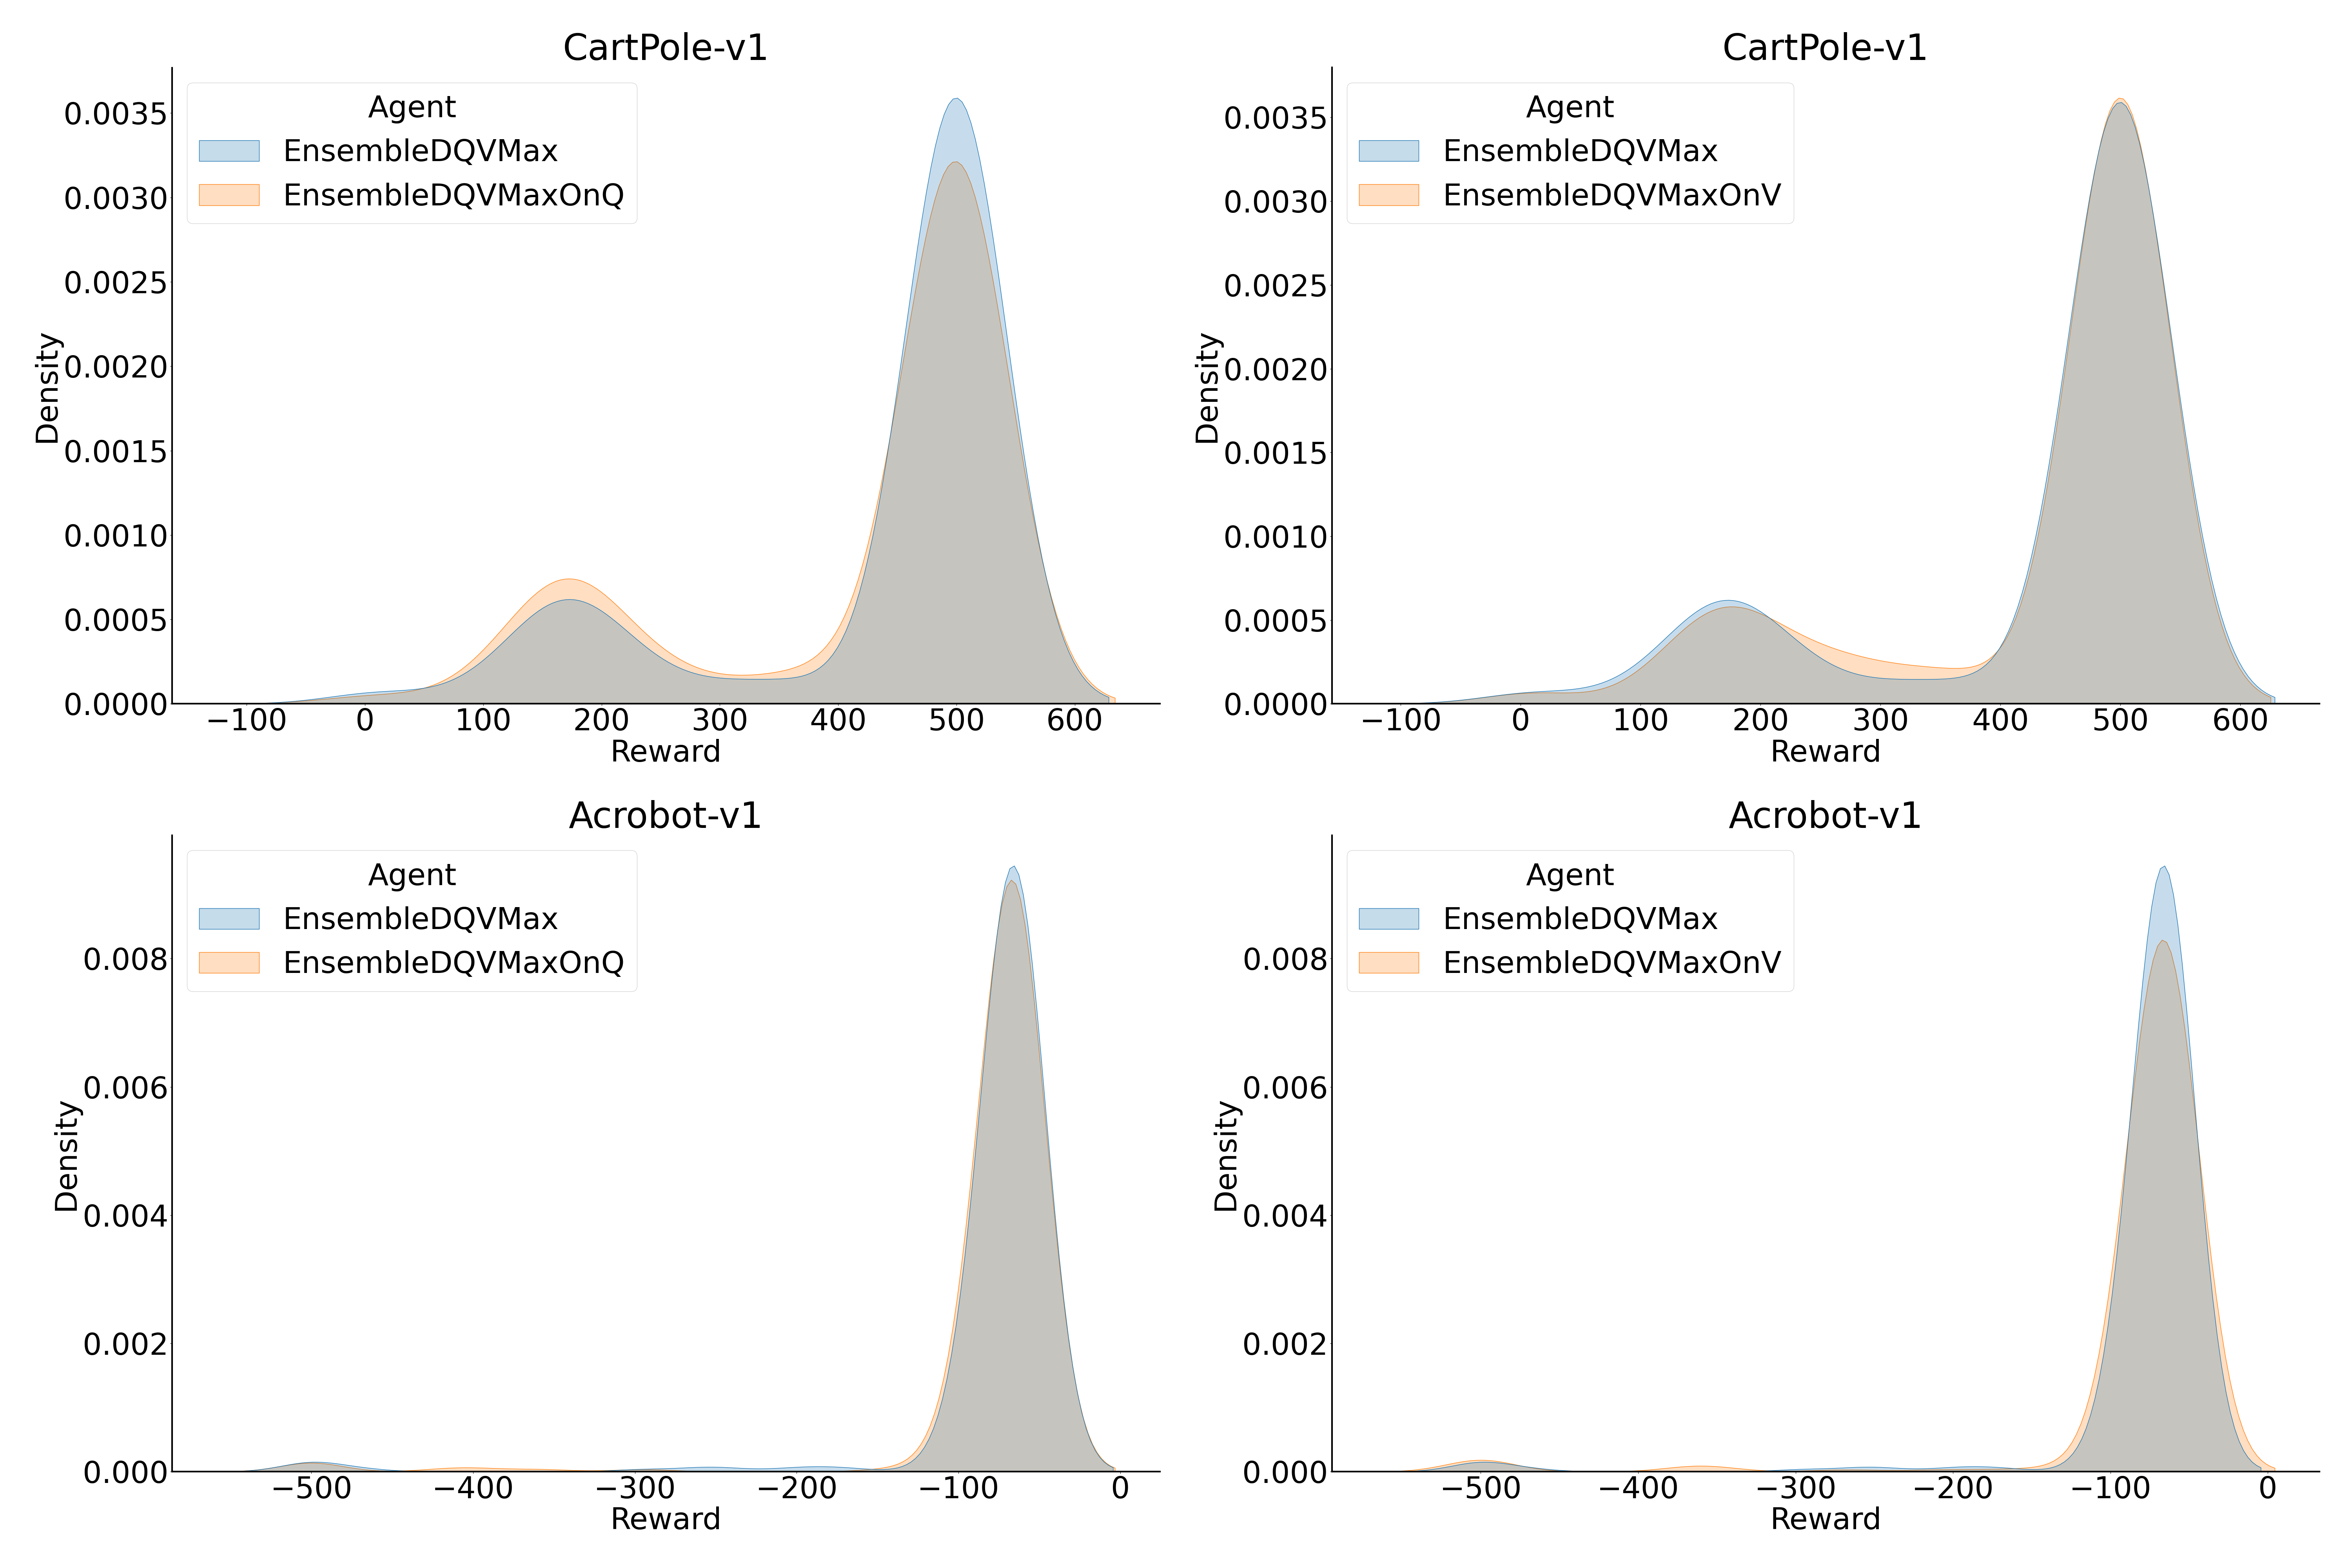
\includegraphics[width=.5\textwidth]{img/dqvmax_abl_rwd_dist.png}
  \caption{Distribution of rewards for Ensemble-DQV-Max compared to
    its ablations}\label{fig:dqvmax_abl_rwd_dist}
\end{figure}

  \newpage
  \subsection{Hyper-parameters}\label{sec:appendix_hparams}

\begin{table*}[t]
\centering
\caption{Hyper-parameters used for online data collection and in the experiments}\label{table:hyperp}
\begin{tabular}{lcc}
\toprule
Hyper-parameter                      & \multicolumn{2}{c}{Value (online and offline)}             \\
\hline
(Training/Evaluation) steps          & \multicolumn{2}{c}{1000}                                   \\
Iterations                           & \multicolumn{2}{c}{500}                                    \\
Redundancy                           & \multicolumn{2}{c}{3}                                      \\
Reward clipping                      & \multicolumn{2}{c}{$[-1,1]$}                               \\
Target network update period (steps) & \multicolumn{2}{c}{100}                                    \\
Discount factor $\gamma$             & \multicolumn{2}{c}{0.99}                                   \\
Exploration strategy                 & \multicolumn{2}{c}{$\epsilon$-greedy}                      \\
Evaluation $\epsilon$                & \multicolumn{2}{c}{0.001}                                  \\
Replay memory size                   & \multicolumn{2}{c}{$500\; 000$ trajectories}               \\
Mini-batch size                      & \multicolumn{2}{c}{32}                                     \\
Replay scheme                        & \multicolumn{2}{c}{Uniform}                                \\
Optimizer                            & \multicolumn{2}{c}{Adam}                                   \\
Adam $\epsilon$                      & \multicolumn{2}{c}{$3.125e-4$}                             \\
Adam learning rate                   & \multicolumn{2}{c}{$0.001$}                                \\
Loss function                        & \multicolumn{2}{l}{Mean Squared ErrorTraining $\epsilon$}  \\
Networks number of layers            & \multicolumn{2}{c}{2}                                      \\
Hidden units per layer               & \multicolumn{2}{c}{512}                                    \\
\hline
Hyper-parameter                      & Online & Offline                                           \\
\hline
Training period (steps)              & 4      & 1                                                 \\
Min. memory size for replay          & 500    & -                                                 \\
Training $\epsilon$                  & 0.01   & -                                                 \\
Evaluation period (iterations)       & -      & 5                                                 \\
\bottomrule
\end{tabular}
\end{table*}

  \newpage
\end{appendices}

\end{document}
